\documentclass[final]{jyflluk}
%\documentclass[draft]{jyflluk}

% Tämä tiedostopohja käyttää biblatexia. JOM (6.3.2016)
\usepackage{graphicx}

\usepackage{caption}
\captionsetup[figure]{format=plain, font=footnotesize, labelfont=bf,labelsep=period}
\usepackage{subcaption}



% Variable "\Otsikko" in LaTeX
\newcommand{\Otsikko}{Microfluidic cancer cell sorting using dielectrophoresis}


%----------------------------------------------------------------------------------------
% LÄHDELUETTELON MUOTOILU
%----------------------------------------------------------------------------------------
\usepackage{csquotes}
\usepackage[backend=biber,style=numeric,sorting=none,maxnames=3,minnames=1,giveninits=true]{biblatex}
\usepackage{xcolor}


\addbibresource{source.bib}

%----------------------------------------------------------------------------------------
% KANSILEHDEN MUOTOILU JA TEKSTI
%----------------------------------------------------------------------------------------
\newcommand*{\titleJYFL}{\begingroup  % Create the command for including the title page in the document
\hbox{                                    % Horizontal box
\hspace*{0.1\textwidth}                   % Whitespace to the left of the title page
\rule{1pt}{\textheight}                   % Vertical line
\hspace*{0.05\textwidth}                  % Whitespace between the vertical line and title page text
\parbox[b]{0.8\textwidth}{                % Paragraph box which restricts text to less than the width of the page

% Tutkielman nimi
{\noindent\LARGE\bfseries \Otsikko\\[0.5\baselineskip]}\\[2\baselineskip]
%
% Tutkielman tyyppi ja päiväys
{\large Master's thesis, \today}\\[3.5\baselineskip]
%
% Tutkielman tekijä 
{\normalsize Author:}\\[0.5\baselineskip] 
{\large \textsc{Peter Balogh}}\\[1\baselineskip]
%
% Työn ohjaajat
{\normalsize Supervisor:}\\[0.5\baselineskip]
{\large \textsc{Andreas Johansson}}
%
% Tyhjä väli ohjaajan nimen ja yliopiston logon välille - älä poista seuraavaa tyhjää riviä!

\vspace{0.2\textheight}
% Yliopiston logo, nimi ja ainelaitos

\includegraphics[height=27mm]{JYU_LOGO.pdf} 
}
}        
\endgroup}
%----------------------------------------------------------------------------------------
% VARSINAINEN DOKUMENTTI
%----------------------------------------------------------------------------------------
\begin{document}
%----------------------------------------------------------------------------------------
% KANSILEHTI
%----------------------------------------------------------------------------------------
\titleJYFL

%----------------------------------------------------------------------------------------
% TIIVISTELMÄ
%----------------------------------------------------------------------------------------
\section*{Abstract}
\addcontentsline{toc}{section}{Abstract}

% Bibliografiset tiedot
Balogh Peter\\ 
\Otsikko\\
Master's Thesis\\ 
Department of Physics, University of Jyväskylä, 2020, \pageref{LastPage}~pages

\bigskip

\textbf{Some filler text, abstract will be done LAST}
\newline
% Tiivistelmän teksti
\noindent Heti opinnäytteen nimiölehden jälkeen sijoitettava tiivistelmä on yhdelle paperille mahtuva ja tavallisesti enintään 250 sanaa sisältävä yhteenveto, joka hyvin tiiviissä muodossa informoi kirjoituksesta. On tärkeää, että tiivistelmä laaditaan huolellisesti, koska sen välityksellä tieto kirjoituksesta leviää eri tietokantojen kautta. Sen tulee olla laadittu niin, että se sellaisenaan voidaan julkaista tietokannoissa. Tiivistelmään alkuun on merkittävä opinnäytteen bibliografiset tiedot ja sen lopussa mainitaan sitä kuvaavat avainsanat. Tiivistelmiä on kahta tyyppiä. Informatiivinen tiivistelmä on tärkein. Se kertoo, mitä ja miten on tutkittu ja mitkä ovat tulokset. Indikatiivinen tiivistelmä osoittaa, mitä kirjoituksessa on käsitelty. Se on sisällöltään yleisempi kuin informatiivinen tiivistelmä, eikä se kerro tuloksista. Tiivistelmän loppuun liitetään aihetta kuvaavat 3--5 avainsanaa helpottamaan tietokantajärjestelmien työtä. Avainsanat voidaan antaa vapaasti asiasisällön mukaan tai poimia termit alan kontrolloiduista sanastoista kuten Yleisestä suomalaisesta asiasanastosta YSA. Opinnäytteen tunnistamiseksi tarvittavat bibliografiset tiedot annetaan tiivistelmän alussa. Tarvittavat tiedot ovat kirjoittajan suku- ja etunimi, opinnäytteen otsikko, opinnäytteen tyyppi, ainelaitoksen nimi, yliopiston nimi, valmistumisvuosi ja työn sivujen lukumäärä (ilman liitesivuja).

\bigskip

% Avainsanat
\noindent Avainsanat: 

%----------------------------------------------------------------------------------------
%	ABSTRACT
%----------------------------------------------------------------------------------------
\section*{Tiivistelmä}
\addcontentsline{toc}{section}{Tiivistelmä}

% Bibliographic information
Peter Balogh\\
\Otsikko \\
Pro gradu -tutkielma \\
Fysiikan laitos, Jyväskylän yliopisto, 2020, \pageref{LastPage}~pages.

\bigskip

% Abstract text
\begin{otherlanguage}{english}
\noindent This should be written in English.
\end{otherlanguage}

\bigskip 

% Keywords
\noindent Keywords: Thesis, abstract, writing, instructions

% --------------------------------------------------------------------------
% ESIPUHE
% --------------------------------------------------------------------------
\section*{Preface}
\addcontentsline{toc}{section}{Preface}

Esipuheen teksti tulee tähän.

\bigskip

Jyväskylässä "DATE HERE"

\bigskip

Peter Balogh

% --------------------------------------------------------------------------
% SISÄLLYS
% --------------------------------------------------------------------------
\tableofcontents

% --------------------------------------------------------------------------
% VARSINAINEN TEKSTIOSA
% --------------------------------------------------------------------------
\section{Introduction}
\label{sec:introduction}

Microfluidics is a field where systems operate with smaller quantities of fluids than nanolitre ($\SI{0.001}{\milli \metre}^3$). Working with such small volumes allows high speed and precise localisation for analysing small particles. Today, microfluidics is mainly used for molecular analysis, but it started off in the 1950’s being a part of ink jet printer manufacturing \cite{gervais_microfluidic_2011}. From there on microfluidics developed after the cold war to field-deployable systems for detection of biological and chemical hazards. In 1980 the rapid growth of molecular biology genomics pushed the development for high throughput DNA sequencing. Finally, the development of the silicon microelectronics contributed with their influence. Photolithography methods could be used to used for microfluidics which allowed further complexity being added on chips, such as electronical detection mechanisms. \cite{whitesides_origins_2006}

Microfluidics give the possibility for cell separation and analysis. Resulting from the small volumes, laminar and high flow speed is achievable. Thus, single cells can be guided through channels and analysis with a high throughput. One important application for this is the separation of individual cancer cells from blood. For cancer treatment, thorough analysis of the cells is required to find out which drugs can work on the specific cancer of an individual. The cells could be screened from blood thus requiring no physical operation, which is important for tumours in difficult areas (e.g. the brain). Fast sorting is required because of their low concentration in blood, circulating cancer cells can be as rare as one in $10^8$ blood cells \cite{huang_enrichment_2013}. This sets the requirement fast analysis; the throughput should be over the kHz range to be practical. 

There are multiple ways for sorting and detecting cells. Optical, thermal, chemical, acoustic, mechanical, magnetic and electrical techniques have been used for cell sorting \cite{ahn_dielectrophoretic_2006,zhang_towards_2015, voldman_electrical_2006}. To differentiate between cells their intrinsic properties, such as size, refractivity or electrical properties can be exploited. One method is to label a cell with a biological marker.  For example, an antibody attached to a fluorophore can label specific proteins or cells selectively. The availability of various biological labels allows cells to be differentiated by fluorescence, radioactivity or by a change in their electromagnetic properties \cite{wilhelm_universal_2008}. Dielectrophoresis is a phenomenon where a force can be exerted on a polarisable particle using a non-uniform electric field. It allows control of unlabelled cells and is the one the fastest sorting methods \cite{zhang_towards_2015}.

A highly popular method for microfluidic device fabrication is “soft lithography”. It includes the use of polymers such as Polydimethylsiloxane (PDMS) to create mold of microstructures. Although it is an inexpensive and fast method capable of creating complex structures like valves and pumps, it has its limitations \cite{xia_soft_1998,tian2008introduction, pethig_review_2010, grover_monolithic_2003}. PDMS can swell because of organic solvents and be damaged \cite{lee_solvent_2003}. Polymers also have limited chemical, mechanical and thermal resistance. In addition, they restrict low wavelength light ($\SI{400}{\nano \metre}$) required for laser induced fluorescence spectroscopy \cite{tian2008introduction,stankova_optical_2016}. Amongst the huge spectrum of microfluidic devices, rarely a pure glass device is manufactured because soft lithography methods being much easier and cheaper. Glass based microfluidics have three main advantages in biological analysis, they are chemically thermally and mechanically stable and are transparent in the visible light wavelength region. The mechanical stability allows to create high pressure, thus high throughput systems. The chemicals stability together with thermal stability allows various solvent usage and cleaning possibility of clogged devices for repeatable use \cite{ofner_high-throughput_2017}. The isolating and heat dissipation properties of glass also allow for high-voltage and frequency dielectrophoretic sorting \cite{effenhauser_high-speed_1994}.
Sorting cells with a $100 \percent$ accuracy \cite{takahashi_non-destructive_2004, thomas_imagebased_2019} or high throughput methods \cite{zhang_towards_2015} have been developed in the past. Sciambi and Abate have even manufactured a device capable of $\SI{30}{\kilo \Hz}$ sorting with over $99 \percent$ accuracy \cite{sciambi2015accurate}. Regardless, high speed together with $100\percent$ accuracy has not yet been shown.

Dielectrophoretic droplet sorting in a glass device has been demonstrated by Ján Borovský for sorting carbon nanotubes at a femtolitre scale \cite{borovsky}. The aim of this thesis is to upscale such a device to be capable of single cell, high throughput, dielectrophoretic sorting. It would be the a part of a microfluidic chip complex, where cells are pre-sorted to higher concentrations using inertial sorting (capable of sorting $\num{3e8}$ cells/s \cite{edd_microfluidic_2020}) and then individual sorting done with dielectrophoresis. Here, the fabrication process  is developed to realise a microfluidic chip suitable for dielectrophoretic sorting using fluorescence spectroscopy. The process is conducted using basic microfabrication methods; e-beam lithography, thin film evaporation, and wet etching.


\section{Theoretical background}
\label{sec:theoretical_background}


\subsection{Microfluidic flow}
\label{sec:subsection1}

Dealing with fluids in the dimensions of micro- to femtolitres characterises microfluidics. The channel diameter that is used to transport the fluid ranges in the micrometre range. These small dimensions grant a benefit over larger volumes. The forces and phenomena dominating at the microfluidic scale differs from its scaled-up counterpart; These are surface tension, diffusion, fluidic resistance and energy dissipation. Out of the many dimensionless numbers that describe the microfluidic environment the most important regarding this thesis will be presented.

Reynolds number $R_e$ describes the ratio of inertial forces to viscous forces in fluids. It is defined as 
%
\begin{equation}
    \label{eq:Reynolds}
    R_e = \frac{\rho u d}{\mu}
 \end{equation}
 %
where $u$ is the flow speed, $d$ is the diameter of the channel, $\rho$ the density and $\mu$ the viscosity of the fluid. The number shows whether the flow described is turbulent or laminar; $R_e$ smaller than 2000 suggesting a laminar flow. Because of the linear dependence of channel diameter microfluidic channels grant typically a low Reynolds number ($R_e$ <1). Laminar flow grants the benefit of precise flow control of the fluid and the particles within. It is possible to flow two different steams of fluid in the same channel without them mixing, allowing the particles to diffuse from one flow to another. \cite{tian2008introduction}

The flow in microfluidic channels can be described by the Poiseuille equation. It describes the pressure drop in a pressure driven flow. It assumes an incompressible Newtonian fluid, which is applicable to microfluidic systems \cite{borovsky}. For a cylindrical pipe, the flow speed is parabolic, slowing down near the edges and increasing towards the centre. The volumetric flow rate Q of a Poiseuille flow can be expressed as
%
\begin{equation}
    \label{eq:Q}
    Q = -\frac{\pi r^4}{8 \mu} \frac{dP}{dz}
 \end{equation}
 %
 where $r$ is the radius of the pipe radius, $\mu$ the fluid viscosity and $P$ is the pressure along the pipe axis $z$ \cite{tian2008introduction}. Although the profile of the manufactured channels in this thesis is different from a circular pipe, this gives an understanding of the features governing the velocity of a laminar flow. For precise flow control the channel dimensions and the inlet/outlet pressures play an important role. 
 Given an incompressible fluid, the microfluidic channels can be modelled by the laws electric currents. The hydrodynamic resistance $R_{hyd}$ of a constant flow rate can be expressed as 
 %
 \begin{equation}
     \label{eq:P}
     \Delta P = R_{hyd} Q
  \end{equation}
  %
 where $\Delta P$ is the constant pressure drop. This can be related to Ohm’s law $U=RI$ and the same type of circuit analysis can be performed to microfluidic channels. At junctions and intersections in Kirchhoff’s laws can be applied, meaning the sum of flow rates entering and leaving any node in the circuit is zero. This means that if the flow is to be divided evenly at a Y-junction, the hydrodynamic resistance of both outgoing channels needs to be the same. \cite{bruus2008theoretical}
 Combining equations \ref{eq:Q} and \ref{eq:P} we can see that $R_{hyd} \propto \mu/r^4$, meaning that the resistance scales unfavourably for a pressure driven flow microfluidic flow. Driving viscous fluids through small channels will require high pressures and correspondingly durable devices.
 
 

\subsection{Fluorescent detection}
\label{sec:x2}
The absorption of electromagnetic radiation into an atom or excites it to a higher energy level. An excited electron returning to its lower energy state will emit its excess energy as a photon. The emitted light is called fluorescence. The electron loses a small amount of energy to vibrational relaxation during the short lifetime of the excited state before emitting a photon and returning to its ground state. This is called the Stokes shift and causes the emitted photon to have a higher wavelength than the exiting one (Figure \ref{fig:atom}). This phenomenon is often used in biology to detect and label cells, cell organelles and even single molecules. Fluorescent molecules (fluorophores) are commercially available with a wide variety of excitation/emission wavelengths, molecular structure, and quantum yield (photons emitted per absorbed ). The main advantage of fluorescence is the shift in emission wavelength. A lower wavelength monochromatic light can be used illuminate the sample whilst only the emitted light is detected by filtering the lower wavelengths (Figure \ref{fig:mic}). Fluorescent labels can have almost $100 \; \percent$ accurate binding specificity and can have increased fluorescence up to an order of magnitude when in the correct binding site or environment (within cell). These labels are organic and deliverable within a cell granting the possibility for live cell labelling and imaging. \cite{toseland2013fluorescent}
 

\begin{figure}[h]
    \begin{subfigure}[t]{0.8\textwidth}
        \centering
            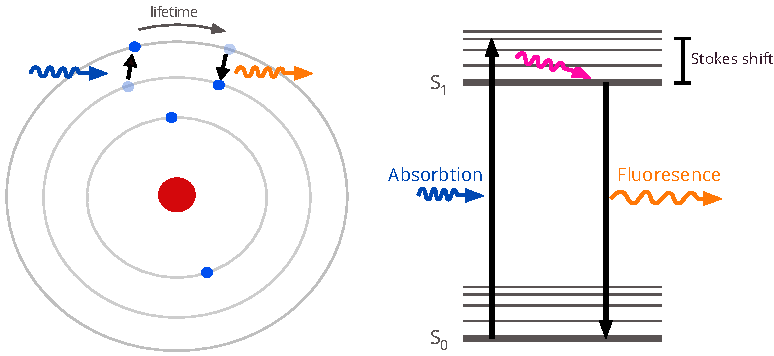
\includegraphics[width=\linewidth]{images/atomm.pdf} 
            \caption{} \label{fig:atom}
        \end{subfigure}
    
    
    \vspace{1cm}
    \centering    
    \begin{subfigure}[t]{0.65\textwidth}
        \centering
        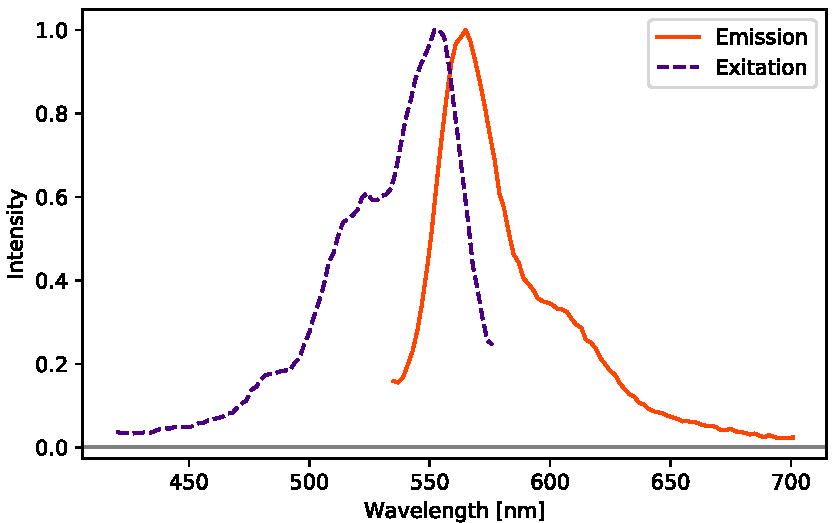
\includegraphics[width=\linewidth]{images/fluore.pdf} 
        \caption{} \label{fig:luo}
    \end{subfigure}
    \hfill
    \begin{subfigure}[t]{0.32\textwidth}
        \centering
        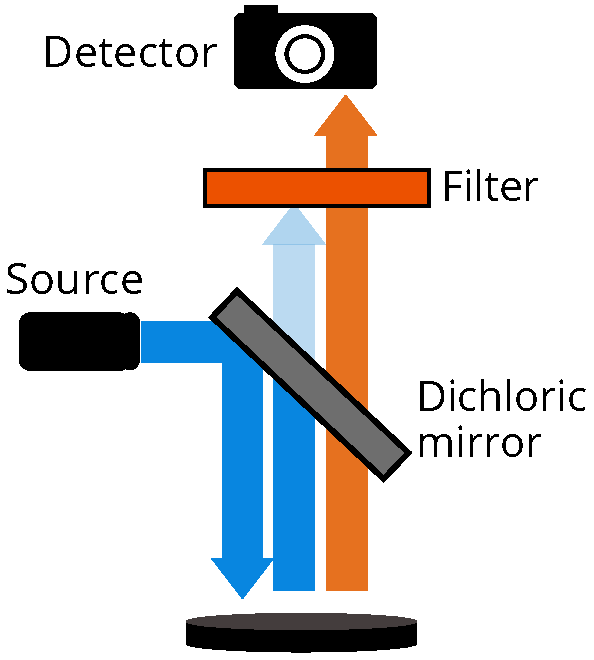
\includegraphics[width=\linewidth]{images/microsco.pdf} 
        \caption{} \label{fig:mic}
    \end{subfigure}
    \caption{a) Basic principle of fluorescence. b) The excitation/emission wavelength of a fluorescent dye (Alexa Fluor 555) as an example. c) The simplified idea of fluoresce imaging.} \label{fig:fluore}
\end{figure}

A characteristic binding site is required achieve targeted protein labelling, but cancer cells include mostly the same proteins as a healthy cell. To distinguish them from normal cells the Warburg phenomenon can be exploited. It is a fundamental characteristic of cancer cells in which fermentation is preferred over phosphorylation as an energy acquiring mechanism \cite{warburg1927metabolism}. As a result, the glucose intake of cancer cells is significantly higher compared to regular cells. Using labelled glucose molecules that are altered to prevent their metabolization, the labelled glucose will accumulate in high-glucose-using cells. This is a common method used in positron emission tomography (PET) scans with a radioactive labels to detect tumours. There are also glucose labels like 2-NBDG (2-[N-(7-nitrobenz-2-oxa-1, 3-diazol-4-yl)amino]-2-deoxy-D-Glucose) which can be used for fluorescent detection of cancer cells \cite{cai20132}. Because of the short lifetime (nano seconds) of the excited state in fluorophores, fluorescence is a suitable method for fast throughput imaging.


\newpage
\subsection{Dielectrophoresis}
\label{sec:x3}
\subsubsection{Theory}
\label{sex:x3.1}

Dielectrophoresis (DEP) is a phenomenon, where a non-uniform electric field can cause a force on a polarizable particle. This phenomenon can be used to move and separate label-free particles. A uniform electric field would cause a uniform charge-distribution on an polarizable particle therefore creating a net-force equal to zero. Respectively, a non-uniform electric field will cause the positive and negative charge accumulation inside the particle to be uneven, causing a net force (Figure \ref{fig:DEP1}b). The direction and the magnitude of the force will depend on the particle’s and mediums polarizability and the electric field \cite{shafiee_contactless_2009}. The term dielectrophoresis was already introduced in 1951 by Herbert A. Pohl \cite{pohl_motion_1951}. It has since gained popularity in microsystems because of its simplicity and favourable scalability $F_{dep} \propto V^{2}/L^{3}$. Here $V$ is the applied voltage and $L$ the distance from particle to electrodes. Meaning, on a smaller system, less voltage is required to achieve the same force $F_{dep}$ \cite{castellanos_electrohydrodynamics_2003}.
\begin{figure}[h]%
    \centering
    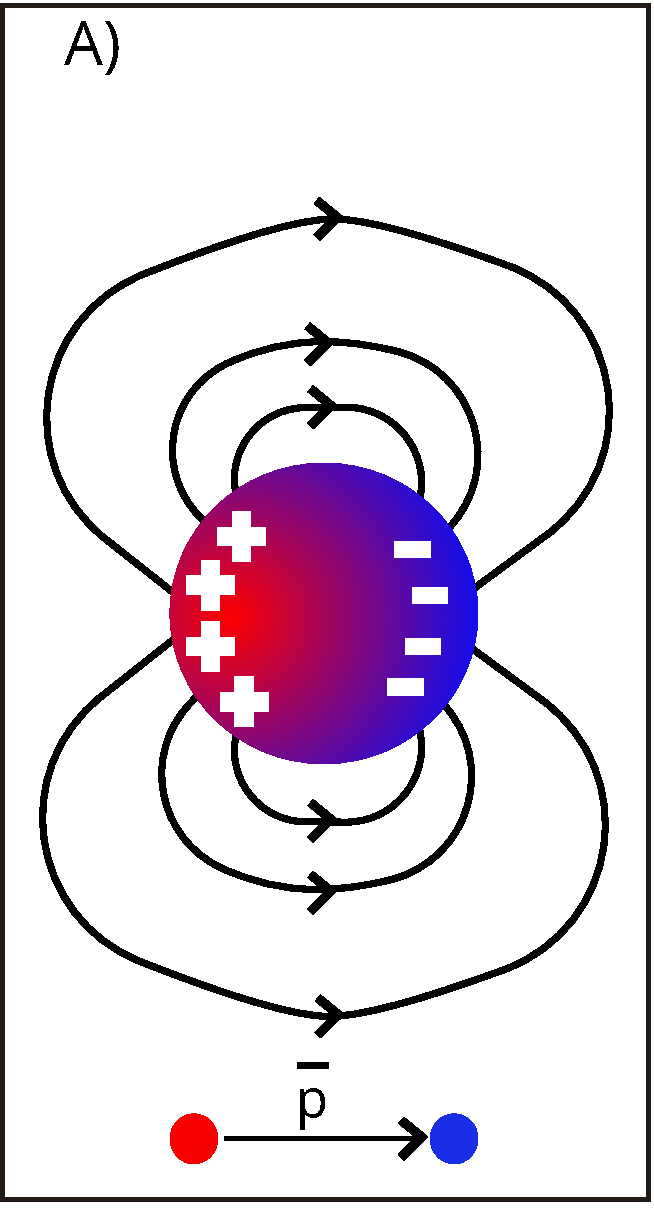
\includegraphics[width=.32\linewidth]{images/pooolar.pdf}\quad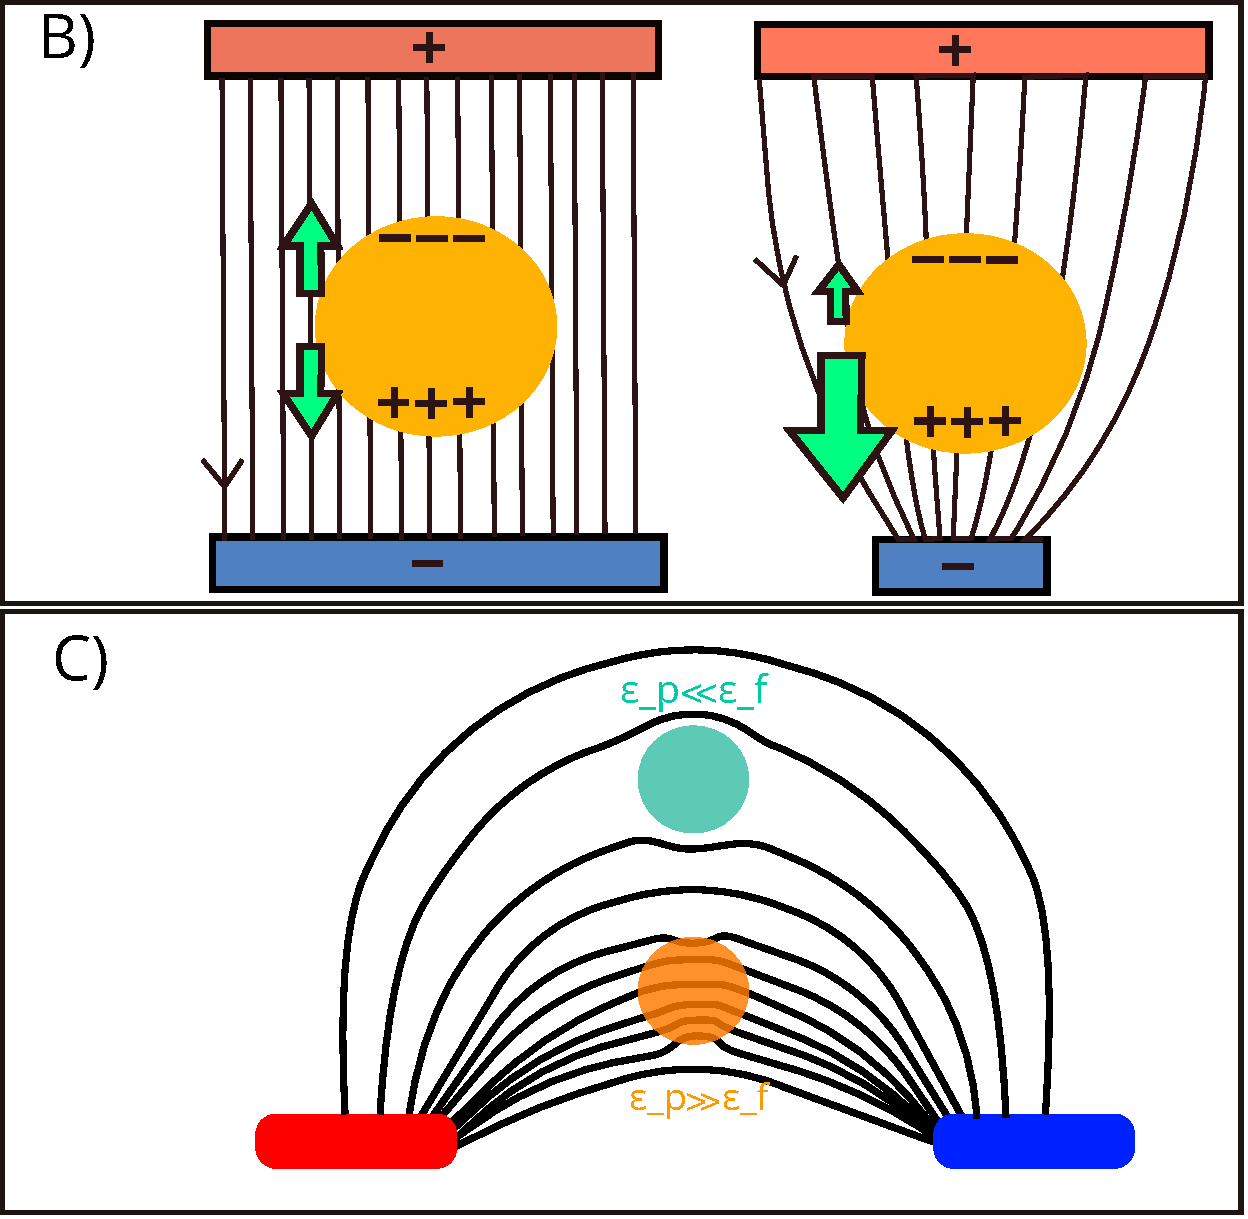
\includegraphics[width=.61\linewidth]{images/merged.pdf}
    \qquad
    \begin{minipage}{1.2in}
    \end{minipage}%
    \caption{Visualisation of DEP. A) A Polarised sphere has a dipole moment B) Net force in a uniform and non-uniform electric field C) Particle and medium permittivity effect on electric field }%
    \label{fig:DEP1}%
\end{figure}

There are multiple mathematical models describing DEP \cite{jubery_dielectrophoretic_2014}. They vary on their complexity and demand on computational power. Here we will be presenting a simplified and general method for the DEP force calculations which has been presented by a number review articles \cite{cottet_mydep_2019, morgan_single_2007,li_review_2014,voldman_electrical_2006}. The force experienced by a dielectric particle can be expressed as
%
\begin{equation}
   \label{eq:F_dielec}
   \vec{F}_{\mathrm{DEP}} = \vec{p} \vec{\nabla} \vec{E}\;,
\end{equation}
%
where $\vec{p}$  is the dipole moment vector, and $(\vec{\nabla} \vec{E})$ the gradient of electric field. The dipole moment depends on the shape of the particle, for a perfect dielectric uniform sphere, it can be expressed as
%
\begin{equation}
   \label{eq:dipmoment}
   \vec{p} = 2 \pi \epsilon_f R^3 \mathrm{Re}[f_{CM}] \vec{E}\;,
\end{equation}
%
Here $R$ is the radius of the particle, $\epsilon_{f}$ the absolute permittivity of surrounding fluid and $\mathrm{Re}[f_{CM}]$ the real part of the Clausius-Mossotti factor (CM) \cite{li_review_2014}. The CM factor for a spherical particle is
%
\begin{equation}
   \label{eq:CM}
   f_{CM} = \left(\frac{\epsilon_{p}^* - \epsilon_{f}^*}{\epsilon_{p}^* + 2\epsilon_{f}^*} \right)\;,
\end{equation}
%
Where and $\epsilon^*$ the complex absolute permittivity of the particle (p) and the surrounding fluid (f). They are related to conductivity $\sigma$ and the angular frequency $\omega=2\pi f$ of the electric field as 
%
\begin{equation}
   \label{eq:complex}
   \epsilon^* = \epsilon - \frac{i \sigma}{\omega}\;,
\end{equation}
%
$i$ being $\sqrt{-1}$. Combining equations (1) and (2) we get and expression for the force
%
\begin{equation}
   \label{eq:F_DEP_norm}
   \vec{F}_{\mathrm{DEP}} = 2 \pi \epsilon_f R^3 \mathrm{Re}[f_{CM}] \vec{\nabla} (\vec{E} \cdot \vec{E}) 
\end{equation}
%
For an AC potential the time average of the force can be expressed as
%
\begin{equation}
   \label{eq:F_DEP}
   \langle F_{\mathrm{DEP}}\rangle = 2 \pi \epsilon_f R^3 \mathrm{Re}[f_{CM}] \vec{\nabla} (E^2_{RMS}) ,
\end{equation}
%
where $E_{RMS}$ is the root mean square value of the electric field $E=\mathrm{Re}[E_0 e^{i \omega t}]$. When the CM factor (Eq.\ref{eq:complex}) is expanded we can see the frequency dependence.
%
\begin{equation}
   \label{eq:CM_open}
   f_{CM} = \left(\frac{(\epsilon_{p} - \epsilon_{f}) + \frac{i}{\omega} (\sigma_f - \sigma_p)}
   {(\epsilon_{p} + 2\epsilon_{f}) - \frac{i}{\omega} (\sigma_p - 2\sigma_f)} \right)\;
\end{equation}
%
Examining the electric field at low  $(\omega = 0)$ or a high frequencies $(\omega = \infty)$ we can see that the CM is reduced to 
\begin{equation}
   \label{eq:wat0}
   f_{CM} = \frac{\sigma_p - \sigma_f} {\sigma_p + 2\sigma_f}, \; \mathrm{when } \;\omega \rightarrow 0 \;
\end{equation}
\begin{equation}
   \label{eq:watinf}
   f_{CM} = \frac{\epsilon_p - \epsilon_f} {\epsilon_p + 2\epsilon}, \;\mathrm{when } \;\omega \rightarrow \infty\;
\end{equation}





At high frequency, the particle acts like a capacitor and is dominated by its permittivity. Whereas, at very low frequencies the current in the particle moves in phase with the electric field thus the conduction is the dominating factor \cite{cetin_dielectrophoresis_2011, li_review_2014, pethig_review_2010}. 
From the CM factor (Eq.\ref{eq:CM}) we can also see that the permittivity of the particle and the surrounding medium determines whether force is pushing or pulling towards the region of stronger electric field. If the particle is more polarizable $(\epsilon_p>\epsilon_f)$ a positive force (pDEP) is pushing towards he higher field and vice versa (Figure \ref{fig:DEP1}c). We can also see from $\epsilon_p>>\epsilon_f$ and  $\epsilon_p<<\epsilon_f $ that the positive DEP force (pDEP) can be twice the magnitude of the negative DEP force (nDEP).
The most important points arising from these equations are:

\begin{enumerate}
\renewcommand{\labelenumi}{\Roman{enumi}}  % <<<<<<<<<<<
    \setlength{\itemsep}{1pt}
    \setlength{\parskip}{1pt}
    \item The Force is zero in a uniform field $(\nabla E=0)$.
    \item The force depends non-linearly on the field magnitude $(E^2)$ and showing that both an AC and CD field can cause a DEP force.
    \item The dependence on particle volume $\propto R^3$ allows separation of particles based on size.
    \item Due to conductivity and permittivity dependence of the medium and particle, the DEP force can be pulling or  pushing. By changing the frequency, there is a crossover-frequency where pDEP changes to nDEP can be achieved. \cite{zhang_dielectrophoresis_2010}
\end{enumerate}
The simplifications made when deriving Eq.\ref{eq:F_DEP} need to be taken into consideration. The particle needs to be a perfect homogeneous dielectric sphere with no net charge. The particles polarisation is assumed as a simple dipole moment, even though a non-uniform field is causing the polarisation.  The medium around the particle is considered infinite and not affected by the particle itself. \cite{pethig_review_2010}

In this thesis the aim is to use DEP for cell sorting. They have various shapes and are not uniform. Cells contain membranes, cytoplasm and organelles. In order to have higher accuracy for simulations more precise mathematical models can be introduced at the cost of computational time \cite{jubery_dielectrophoretic_2014, cetin_dielectrophoresis_2011, pethig_review_2010, cottet_mydep_2019}. But, even with its simplifications, this model is sufficient to describe the our DEP system because the underlying physics are present.

\subsubsection{Single shell model}
\label{sec:x3.2}

The CM factor for a mammalian cell has characteristic properties. For example, a white blood cell has been demonstrated \cite{voldman_electrical_2006}. At low frequencies ($<\SI{100}{\kilo \Hz}$) the cell is less polarizable than a typical ionic solution thus causing a nDEP effect. Similarly when going to MHz frequencies, the conductivities of the solution and the cell will matter more, thus resulting in a pDEP in low conductivity solutions ($\SI{5.5e-6}{ \siemens \per \metre}$ for Di water \cite{pashley2005gassed}). At GHz range, the the permittivities will be mainly compared (Eq.\ref{eq:watinf}) and likely to cytoplasmic proteins, the permittivity of the cell is low compared to water and results in a negative dep.  Although the frequency depends highly on the cell and medium properties, the “single-shell” model (Figure \ref{fig:single_shell}) predicts this two times cross over frequency \cite{cetin_dielectrophoresis_2011,pethig_review_2010, voldman_electrical_2006, cottet_mydep_2019}. The single-shell model uses a CM factor where a shell (cf. cell membrane) is accounted for with its own properties. In the single shell model the complex permittivity is
%
\begin{equation}
   \label{eq:shellmodel}
   \epsilon^*=\epsilon_{mem} \left[ \frac{\left( \frac{r}{r-d}\right)^3 + 2\left(\frac{\epsilon_{CP}^* - \epsilon_{mem}^*}{\epsilon_{CP}^* + 2\epsilon_{mem}^*} \right)}{\left( \frac{r}{r-d}\right)^3 -\left(\frac{\epsilon_{CP}^* - \epsilon_{mem}^*}{\epsilon_{CP}^* + 2\epsilon_{mem}^*} \right)}        \right] \;,
\end{equation}
%
where $r$ , $d$ the thickness of the membrane, $\epsilon_{CP}^*$ and  $\epsilon_{mem}^*$ are the complex permittivities of the cytoplasm an the membrane. A simulation of the CM factor using the single shell model for HT-29 cells is shown in Figure \ref{fig:single_shell}. The result is from a Java  simulator published by Cottlet et Al \cite{cottet_mydep_2019}.

\begin{figure}[h]%
    \centering
    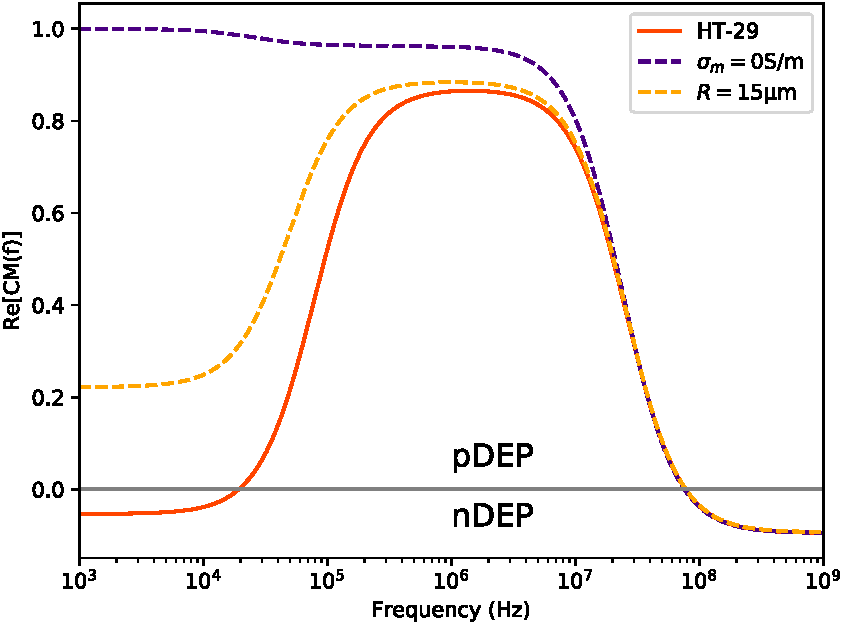
\includegraphics[width=.70\linewidth]{images/plot_DEP2.pdf}\quad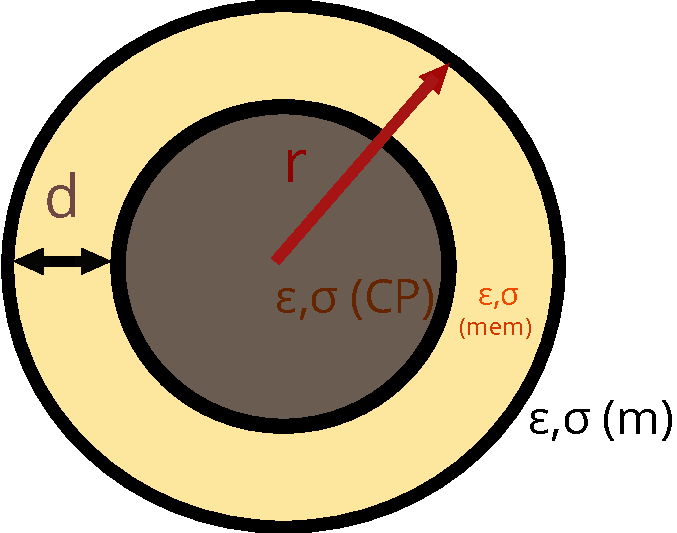
\includegraphics[width=.27\linewidth]{images/single_shell.pdf}
    \qquad
    \begin{minipage}{1.2in}
    \end{minipage}%
    \caption{(Left) CM factor for Human colon cancer cells (HT-29) has been simulated with MyDEP tool \cite{cottet_mydep_2019}. The values used in the simulation are presented in table \ref{tab:cell_table}. A change in cell radius and a change in media was also simulated for comparison. (Right) The single shell model.}%
    \label{fig:single_shell}%
\end{figure}


For comparison, a simulation was also done with the same cell having a larger radius and one being submerged in DI-water $(\sigma_{DI}\approx0)$. In reality, the change in medium conductivity can affect the membrane conductivity up to 2 orders of magnitude, which has not been accounted for in this simulation \cite{wu_dielectrophoretic_2012}. This simulation gives a sense for order of magnitude of the frequency to be used in our experiment. It also shows that cells with different properties, such as size, electrical properties and shape, can be separated with DEP with a correct frequency. Around the crossover frequency cells can experience nDEP or pDEP depending on their properties. Separating cancer cells from blood using DEP has already been demonstrated by multiple publications \cite{becker_separation_1995,huang_enrichment_2013,kang_continuous_2006, ivory_direct_2011}.

\begin{table}[h]
   \centering
   \caption{The literacy values for HT-29 Human colon cancer cells \cite{wu_dielectrophoretic_2012}.}
   \label{tab:cell_table}
   \begin{tabular}{cccccc} \toprule
      $\sigma_m$ (S/m)    & $\epsilon_{mem}$ & $\epsilon_{mem}$ & $\sigma_m$ (S/m) & $\sigma_m$ (S/m) & $R$ ($\mathrm{\micro\metre})$\\ \midrule
      $0.01$              &  $4.68$        &  $68.31$       & $6.63e-6$        & $0.279$          & $6.6$\\
        \bottomrule
   \end{tabular}
\end{table}


\subsubsection{Choosing DEP}

For successful high throughput cell sorting, the correct parameters are needed to be chosen to our DEP system by accounting for all the challenges and advantages. The electrodes for DEP can be manufactured to be in contact with the sample fluid or contactless. DEP can be achieved using AC or DC currents. The field strength can be chosen by varying the potential or the dimensions of the electrodes. For nDEP or pDEP the correct frequency needs to be chosen for the AC alternative. As an outcome, the DEP force needs to out scale drag force, buoyancy force, electrothermal forces and Brownian motion (not a problem for >1um particles) \cite{cetin_dielectrophoresis_2011}.

For DEP applications, the most common way is placing the electrodes in contact with the liquid. This allows the particles to be closer to the electrodes thus perceiving a higher gradient which allows for better control precision. \cite{voldman_electrical_2006}. Unfortunately, contact with the sample fluid can lead to many problems, especially with biological samples. Electrode polarization, dissolution, bubble formation, contamination of the fluid and fouling can affect the operation. Especially in DC systems electrochemical effects can produce $\mathrm{H_2}$ and $\mathrm{O_2}$ gas. Joule (resistive) heating causes a problem, already at $4\celsius$ above body temperature ($37\celsius$) it can lead to mammalian cell death. \cite{voldman_electrical_2006,cetin_dielectrophoresis_2011,shafiee_contactless_2009}.
Using contactless electrodes, bubble formation, contamination and  fouling are completely eliminated. The medium is then only in contact is the substrate. This also reduces heating from a high intensity light, e.g. Fluorescence inducing light, absorbed by the electrodes. For contactless electrodes AC is the better choice, because DC would require higher voltages for sufficient DEP, which leads to joule heating. A high frequency electric field is also less stressing on a cell membrane, which have voltage sensitive proteins, than that of a DC field \cite{voldman_electrical_2006}.























































%%%%%%%%%%%%%%%%%%%%%%%%%
%%%%%%%%%%%%%%%%%%%%%%%%%
%%%%%%%%%%%%%%%%%%%%%%%%%


\section{Methods}
\label{sec:methods}

\subsection{Cleaning and activation}
\label{sec:xx1}

Cleaning the glass chips before the fabrication steps is of critical importance. Most of the process steps require dust/particle contaminant free surfaces. The two main reasons are for good thin film adhesion and thermal bonding. Surface contaminants cause bad adhesion and pinholes in thin films. In thermal bonding of the chip and the cover-glass, they cause Newton-rings. Around the contaminant colourful ring shape can be perceived resulting from the opening between the two glass surfaces. This opening can lead to leakage and destruction of the chip.
Cleaning the glass was done by scrubbing the surface with cotton tips in acetone, then sonicated and rinsed in Isopropyl Alcohol (IPA). Acetone is a good organic solvent for general cleaning, removing fingerprints and dissolving glue from tape residue. The mechanical scrubbing together with sonification loosens and removes solid contaminants. The final rinse with IPA removes the traces of acetone and evaporates quickly leaving a spotless surface. To ensure cleanliness, the glass can be dried with $\mathrm{N_2}$ blowing and checked against light for contamination.  To minimize particle contamination the chips should be transported in deionised water. Despite being in a cleanroom, ambient air is a potential risk for contamination. 
For the removal of metal and organic contamination and glass surface activation, Piranha solution was used \cite{franssila2010introduction}. Piranha is a strong oxidizing agent consisting of sulfuric acid ($\mathrm{H_2 SO_4}$) and hydrogen peroxide ($\mathrm{H_2 O_2}$). The ratio can be tuned, but if the concentration of $\mathrm{H_2 O_2}$ is over $50 \percent$ an explosion can occur \cite{piranha2014}. The solution is heated to $\SI{100}{\celsius}$ to increase the reaction speed but only after it is cooled after mixture because the reaction is highly exothermic. The solution also hydroxylates glass surface (Activation) adding -OH groups \cite{klug2013chemical}. The hydroxylation helps thin-film adhesion and is necessary for the bonding of glass. Surface activation can also be achieved with RIE (Reactive Ion Etching)\cite{lazauskas2012float}. High frequency $\mathrm{O_2}$ plasma treatment can also remove contamination and  hydroxylate the glass surface. It is a faster method compared to Piranha clean but is not as effective than the highly reactive aforementioned chemical clean.









\subsection{Thin film deposition}
\label{sec:xx2}


\subsubsection{Evaporation}

The etch mask quality is crucial for etching, thus it is important to understand the deposition mechanism to fix film quality problems. Thin film deposition on a substrate is one of the key methods in microfabrication dating back to the 19th century \cite{ohring1992materials}.  Today, the production of thin films has been mastered mainly for the needs of the semiconductor industry. Thin films can become a permanent part of the substrate (e.g. electrodes, semiconductors, capacitors, insulators or protective elements) or act as etch masks \cite{franssila2010introduction}. One of the many methods of producing thin films on a substrate is evaporation, where the material is evaporated from liquid form or sublimated. When the evaporated material hits a cooler surface it will deposit, forming an amorphous film. Evaporation requires the vapour pressure to be higher than of its surroundings. Naturally, there are two ways to achieve this; Either the material’s vapour pressure is increased by heating or the surrounding gas is vacuumed. The evaporation rate $\phi$ (flux of the material) can be expressed using the vapour pressure $P_V$ as 
%
\begin{equation}
    \label{eq:fluxx}
    \phi = \frac{P_v (T)}{2 \pi m k_b T}
 \end{equation}
where $k_b$ is the Boltzmann constant, $m$ the mass, and $T$ the temperature of the material \cite{franssila2010introduction}.

\subsubsection{E-beam evaporation}

The method used in this thesis was Electron-beam physical vapor deposition (EBPVD) or E-beam evaporation for short. In EBPVD the kinetic energy of electrons is used to heat the target material. An electron source is created by joule heating a tungsten ($\SI{3660}{\kelvin}$ melting point) filament to cause thermionic emission \cite{franssila2010introduction}. The released electrons are then accelerated by an applied voltage and guided into a crucible using a magnetic field (Figure \ref{fig:evaporator}). The Kinetic energy of the electrons heat the target material leading to its evaporation. When the correct evaporation rate is achieved, a shutter covering the substrate is removed allowing the evaporated material to deposit on the substrate.


\begin{figure}[h]
    \centering
    \begin{subfigure}{0.56\textwidth}
        \centering
        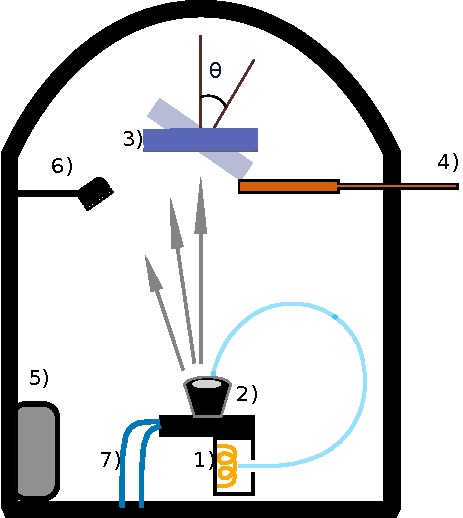
\includegraphics[width=\linewidth]{images/evaporatorr.pdf} 
        \caption{Evaporator} \label{fig:evaporator}
    \end{subfigure}
    \hfill
    \begin{subfigure}{0.35\textwidth}
        \centering
        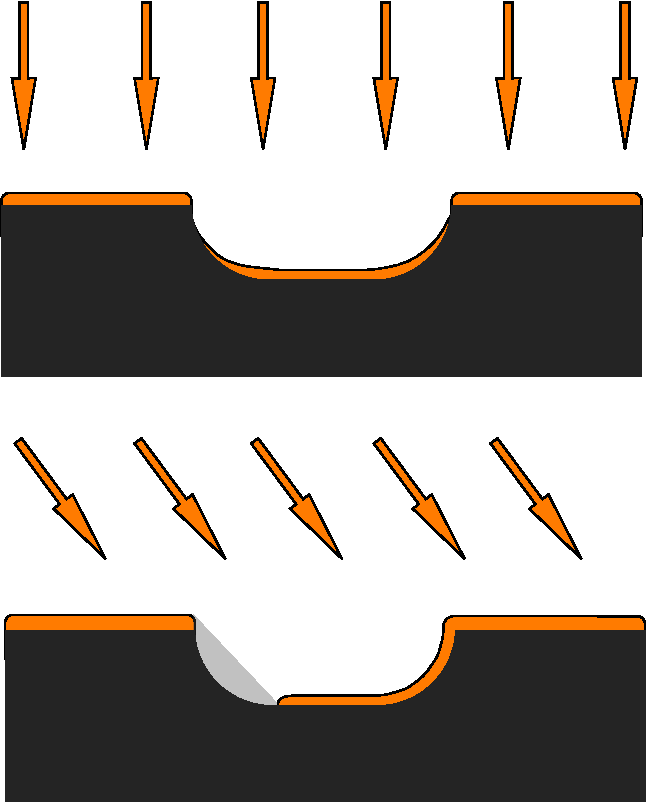
\includegraphics[width=\linewidth]{images/angle_evap.pdf} 
        \caption{Line of sight coverage} \label{fig:angle_evap}
    \end{subfigure}
    \caption{a) Schematic of an e-beam evaporator. 1) Electron source 2) Crucible containing the target material 3) Substrate with variable angle 4) Shutter 5) Pump 6) Thickness detector 7) Water cooling. b) Comparison of direct and angle evaporation. } \label{fig:evap}
\end{figure}



The biggest concern in thin film deposition is contamination. Impurities can cause bad film adhesion, pinholes and change in chemical composition of the film rendering it useless for its applications. The main sources for contamination arise from impurities in the evaporation material, the crucible, cleanliness of the chamber, or the gases present in the evaporation chamber. Evaporation materials are usually sold with high purity (over $99.99 \percent$), but they easily contaminate if stored unproperly. In example Chromium oxidises quickly when in ambient air. 

To avoid the evaporated material colliding with gas molecules, their mean free path should be longer than the distance from crucible to substrate. The mean free path $\lambda$ can be derived from the kinetic theory of gases to be 
%
\begin{equation}
    \label{eq:mean_free}
    \lambda = \frac{k_b T}{\sqrt{2}\pi d^2 P}
 \end{equation}
$T$ being the temperature, $P$ the pressure and $d$ the effective cross-section of the particle. In an ideal case, the evaporated material travels directly to the substrate. The main advantage of using an EBPVD is that the beam heats only the target material and not the crucible. Keeping the crucible at lower temperature prevents the evaporation of the crucible itself or unwanted chemical reactions between the crucible and the material. The localised heating allows evaporation of even tungsten. \cite{franssila2010introduction}

Collisionless transport results in a line of sight coverage which can lead to non-uniform film thickness. The thickness uniformity depends on the position of the substrate to the source. The substrate edges being in a different angle or distance from the source will result in a different film thickness compared to the centre of the substrate. Small thickness variations are not important parameters for an etch mask, for that, the coverage is crucial. It can be influenced by the evaporator design. A longer distance between source and substrate, rotation and angle variation of the substrate can all affect the coverage (Figure \ref{fig:angle_evap}).
To produce pure films, a low pressure in required with a high deposition rate \cite{ohring1992materials}. The deposition rate can be tailored by increasing the acceleration voltage of the electrons and hence the temperature of the target material. The rate can be measured inside the chamber with almost atomic layer precision by using a quartz crystal. The deposited mass on the crystal changes its resonant frequency, which can be precisely measured \cite{franssila2010introduction}. 

Before evaporation, adhesion and stress of the film should be considered. Unless special combinations of substrate and evaporation materials are picked, the adhesion will be poor. If the film material isn’t compatible with the target surface, adhesion layers can be used. Noble metals like Gold aren’t reactive and will not form metal-oxide bonds with, which are a necessity for good oxide surfaces adhesion. In example the adhesion between Gold and glass is very poor. A strong adhesion can be achieved with the use of $\mathrm{TiW}$, $\mathrm{Ti}$ or $\mathrm{Cr}$ adhesion layers, with a few nanometres of an adhesion layer being sufficient \cite{chen2013study}. Substrate cleanliness is the next important factor for film adhesion because impurities will not allow bond formation. Internal stress of the film will weaken the adhesion. Although evaporated films do not suffer from stresses arising from a crystal structure, it does experience tensile stress from temperature difference.  Therefore, some evaporators have the possibility to heat the substrate. \cite{franssila2010introduction}

\begin{figure}[h]
    \centering
    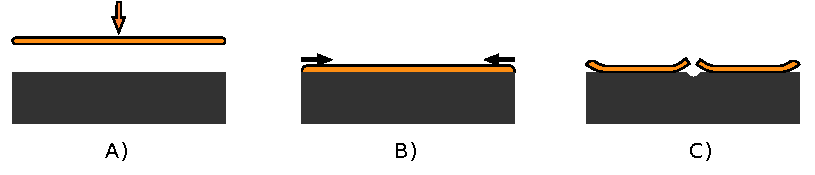
\includegraphics[width=1.0\textwidth]{images/tensile.pdf}
    \caption{Tensile stress in evaporated thin-films. a) When evaporated, the target material is hot. b) Deposition on a cool substrate will lead to stress from thermal expansion. c) If a hole is made in the film (by pinhole or etching) the stress will bed the film from the surface.}
    \label{fig:stresa}
\end{figure}

\subsection{E-beam lithography}
\label{sec:xx3}

The idea of lithography is print a pattern on a surface by changing the surface properties.  Photolithography is indeed the main method used in microfabrication. The idea is to use a photosensitive material (resist) and expose it to light through a mask, that allows light to penetrate only at desired areas. The exposed areas undergo a chemical reaction which is used to generate a pattern. The exposed areas (positive resist) or the unexposed areas (negative resist) can be then chemically removed (Figure \ref{fig:SEM}).  Photolithography serves well the microfabrication industry, because hundreds of copies can be printed using a single mask. Photolithography is the most popular method in microfabrication. The drive to imprint smaller features (Moore’s Law) has led to the development new methods.
\cite{franssila2010introduction, lee2010microfabrication}


\begin{figure}[hb]%
    \centering
    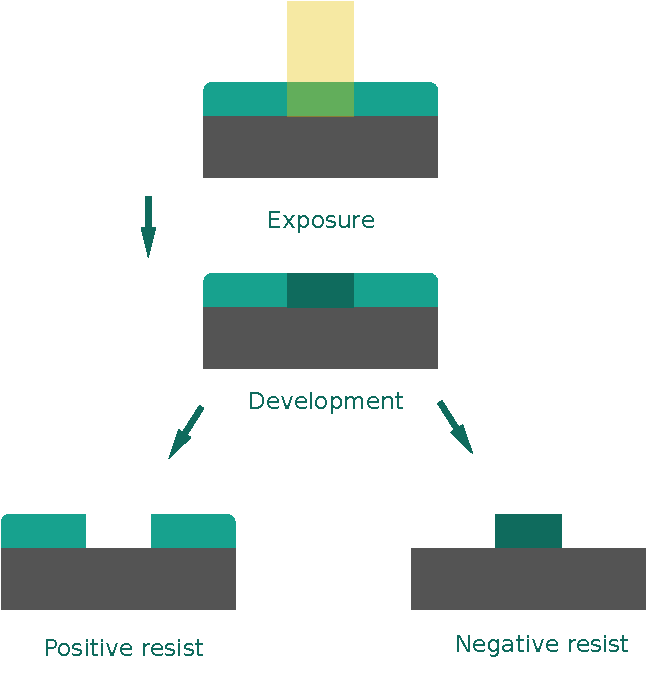
\includegraphics[width=.40\linewidth]{images/pos_neg_resist.pdf}\quad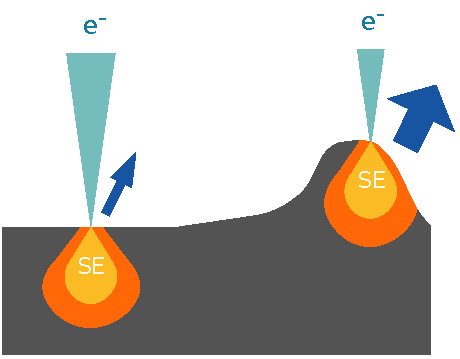
\includegraphics[width=.43\linewidth]{images/SE.pdf}
    \qquad
    \begin{minipage}{1.2in}
    \end{minipage}%
    \caption{(Left) Positive and negative resist exposure and development (Right) SE generation. SE's can can escape from close to surface, an inclined surface will produce more SE's thus increasing the contrast.}%
    \label{fig:SEM}%
\end{figure}

\subsubsection{Electron microscope}

Electron microscopes were developed to overcome the resolution of optical microscopes, which were limited by visible lights diffraction. The first Scanning Electron Microscope (SEM) was built by Max Knoll in $1935$ \cite{oatley1982early}. SEM follows the basic principles of an electron microscope. This means that it contains an electron source, usually a tungsten filament which emits electrons via thermionic emission when a sufficiently high voltage (\numrange[range-phrase = -]{100}{300} kV) is applied. Much like in optical microscopes the beam is then focused, but by the magnetic field of coils. SEM is not limited by the diffraction limit because of the small wavelength of electrons. Combining the de Broglie wavelength $\lambda = h/mv$ with kinetic energy $E_{kin} = 1/2 mv^2$, we can get an expression for their wavelength as 
\begin{equation}
    \label{eq:wavelength_electron}
    \lambda = \frac{h}{\sqrt{2 m E_{kin}}}
\end{equation}
where $h$ is Planck's constant and $m$ the mass of an electron. The electrons can be accelerated by an applied electric field acquiring an energy of \numrange[range-phrase = -]{10}{100}$\;\kilo \electronvolt$ \cite{EBL_GOOD}. An electron with a kinetic energy of $\SI{20}{\kilo \electronvolt}$ would have a wavelength of $\SI{8.7}{\femto \metre}$. The electron beam is focused to an area of \numrange[range-phrase = -]{0.4}{5}$\;\nano\metre$ (pixel size) and the sample is raster scanned. Each pixel is then analysed separately, and the data recorded.  

SEM uses mainly the detection of secondary electrons (SE) which have lower kinetic energies than the backscattered ones. The SE emission is caused near the sample surface due to inelastic scattering, produced by ionisation. SE’s can escape the sample only from near the surface thus revealing information about the sample topology (Figure \ref{fig:SEM}). At a sharp profile, SE emission is increased leading to increased electrons in the detector, resulting in a brighter pixel. E-beam lithography has the same principle as photolithography, but instead of photons, the resist is exposed to electron bombardment which can be achieved with an electron microscope. When using a SEM, the sample needs to be able to withstand the vacuum inside the microscope. It also needs to be somewhat conducting to avoid accumulation of electrostatic charge.


\subsubsection{Resists, PMMA}

Resists consist of carbon-based polymer chains that react to electromagnetic wave exposure. As in photoresists the chemical reaction in e-beam resists is either the cross-linking or fragmentation of chains. In a positive resist the polymer chains are disrupted making them shorter, which can dissolve easier in an organic solvent (developer) (Figure \ref{fig:PMMA_chem}). Likewise, in negative resist longer chains are formed, thus making the exposed areal less soluble. One of the first developed and the most popular e-beam resist is Polymethyl methacrylate (PMMA). It has the capability of acting as both positive and negative resist. PMMA is highly sensitive (requires little exposure compared to other e-beam resists) and has a resolution of $\SI{10}{\nano \metre}$ but it has poor etch resistance. For the development of PMMA, MIBK:IPA (Methyl isobutyl ketone: Isopropyl alcohol) is used and for removal, Acetone. \cite{EBL_GOOD}

\begin{figure}[h]
    \centering
    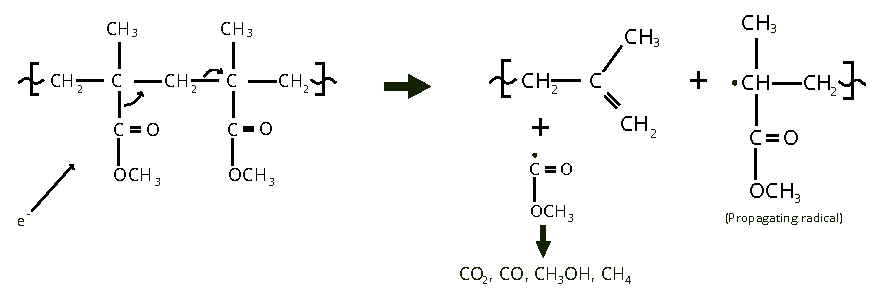
\includegraphics[width=1.0\textwidth]{images/PMMA_chem_eq.pdf}
    \caption{The mechanism of PMMA polymer scission due to e-beam exposure. Adapted with permission from \cite{moore_degradation_1991}. Copyright 1991 American Chemical Society.}
    \label{fig:PMMA_chem}
\end{figure}

Selection of the correct resist is important for achieving the desired result. Multiple resists are available with different sensitivities, contrast and developers. The composition of the resist itself can also be varied. For example, both PMMA 950K A4 and -A11 were used in this thesis.  950K refers to the molecular weight and “A” to the solvent ($4 \percent$ PMMA in Anisole). To achieve a good lithographic process these parameters should be optimized:
\begin{enumerate}
    \renewcommand{\labelenumi}{\Roman{enumi}} 
    \setlength{\itemsep}{1pt}
    \setlength{\parskip}{1pt}
        \item Exposure dose
        \item Development time
        \item Resist adhesion to substrate
        \item Resist thickness
\end{enumerate}	
In the case of a glass substrate solely PMMA cannot be used. It is not conductive and  will cause charge accumulation, which will have a repelling effect on the incoming electrons. Charge accumulation will lead to unwanted exposure areas, ruining the sample. Usually a thin metal film or a layer of conductive resist is used to ground the sample.




\subsection{Wet etching}
\label{sec:xx4}

Etching is the subtractive process in microfabrication. Material is etched in order to create cavities, patterns or just to remove unwanted material. Etching can be divided into physical or chemical methods. Physical methods consist of eroding the material, in example, with a focused ion beam. Chemical etching is based on chemical reactions removing the material. 

In wet etching the substrate is simply dipped into a chemical solution which will react with the target material. In most cases a mask is used to allow the chemical reaction to happen only at the desired areas. When choosing an etchant, selectivity is the key factor. The aim is to have the etchant reacting specifically with the target material leaving the mask and other materials unspoilt. A faulty or deteriorated mask will lead to the destruction of the sample. 
Wet etching is a highly tuneable process. Chemical information and reactions of different etchants are widely available thanks to the microfabrication industry \cite{williams2003etch}. After finding the correct etchant, the etch rate can be tuned by etchant concentration, temperature and stirring. Compared to physical etching wet chemical etching is faster. The drawback of wet etching is isotropy. Because the etchant etches ideally in all directions, the target material will be etched from the mask opening as much in depth as in the lateral dimension, meaning the ratio of depth:width will always be at least 1:2 (Figure\ref{fig:isotropy}). In reality the etch rate can vary in the lateral direction due to the availability of fresh etchant in small cavities. \cite{lee2010microfabrication}
\begin{figure}[h]
    \centering
    \hspace*{1cm}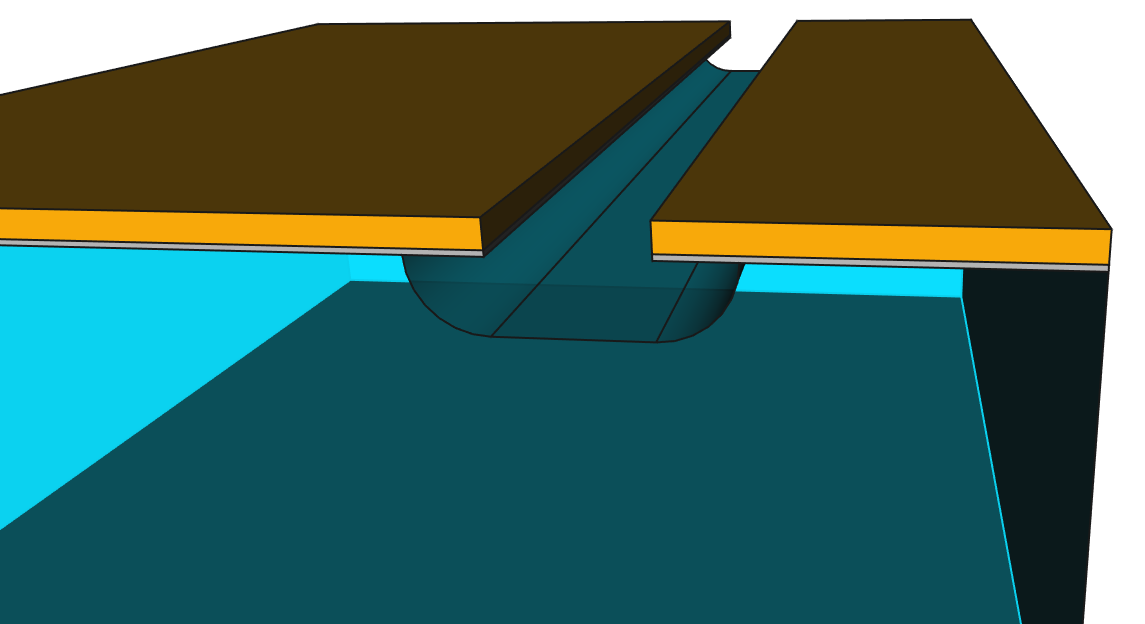
\includegraphics[width=0.6\textwidth]{images/isotrpy.png}\hspace*{-1cm}
    \caption{Isotropic etching. The etch rate from the mask opening is the same in all directions.}
    \label{fig:isotropy}
\end{figure}
\newline
\newline
\textbf{Glass etching}

Wet etching of glass is difficult due to its chemical stability, it is mainly etched with hydrofluoric acid (HF). The generalised etch mechanism is reportedly \cite{etch_formula}
\begin{equation}
    \label{eq:HF_etch}
    \mathrm{SiO_2} + \mathrm{6HF} \rightarrow  \mathrm{2H_2 O} + \mathrm{H_2 Si F_6}
\end{equation}

The challenge with HF is that it is a highly dangerous chemical and for safety reasons, boiling and sonication is not recommended. Additionally, only a few mask materials are chemically inert to it.  Using a solely a photoresist as mask for HF etching has been reported \cite{lin2001fast,guanglong2012microfluidic}, but the most common mask for HF glass etching is the combination of Au and Cr, which are both inert to HF \cite{iliescu2005characterization,tay2006defect}. Other combinations like WTi/Cu and Cr/Cu have also been demonstrated as being able to act as a masking material \cite{Hgglund2013CharacterizationOM,iliescu2008wet}.
From equation \ref{eq:HF_etch} we can see that the reaction depends highly on the concentration of HF. But the formula is applicable only for pure quartz glass. The glass used in this thesis was Soda Lime, which was chosen because of its low cost and high etch rate compared to other glasses \cite{srivannavit2004design}. It consists of multiple components which are presented in Table \ref{tab:soda_lime}. 
\begin{table}[h]
    \centering
    \caption{The composition of soda-lime glass slides according to manufacturer \cite{Soda_lime_ONLINE}.}
    \label{tab:soda_lime}
    \begin{tabular}{cccccccc} \toprule
       $\mathrm{SiO_2}$  & $\mathrm{MgO}$   &  $\mathrm{Na_2 O}$ & $\mathrm{Al_2 O_3}$ &  $\mathrm{K_2 O}$ &  $\mathrm{Fe_2O3}$ &  $\mathrm{CaO}$ & $\mathrm{SO_3}$ \\ \midrule

       $72.20 \percent$  &  $4.30 \percent$ &  $14.30 \percent$  & $1.20 \percent$     &  $1.20 \percent$  & $0.03 \percent$    & $6.40 \percent$ & $0.30 \percent$\\ \bottomrule
    \end{tabular}
\end{table} 
$\mathrm{CaO}$, $\mathrm{MgO}$ and $\mathrm{Al_2 O_3}$ can form insoluble products together with HF, and they can leave precipitations and create “masked” areas for the etchant, which will result in a rough surface. Mixing HCl has proved to dissolve these molecules and result in a better etch surface \cite{iliescu2005characterization}. The etch rate and surface roughness quality can be further tuned by the addition of $\mathrm{HNO_3}$, $\mathrm{H_3 PO_4 }$  or $\mathrm{H_2SO_4}$ \cite{park2017review}. In the case of Deep etching (over $\SI{10}{\micro \metre}$) high etch rates are desirable. There is always a probability for mask defects and the etchant penetrating them. The penetration of the etchant through these defects is constant, so reducing the etch time by having a high etch rate will result in less defects \cite{tay2006defect}. Other than glass composition, etchant concentration and applied heat the etch rate can be increased by annealing the glass. Annelaing reduces stress and redistributes oxides within the glass, leading to a stable etch rate throughout the glass \cite{iliescu2005THOROUGH}.





\label{sec:xx5}
\subsection{RIE}
Reactive ion etching (RIE) is a dry chemical and physical etching method where a reactive plasma is used to etch material. In RIE, the substrate is placed within a vacuum chamber, which is then filled with a suitable reactive gas. A capacitively (or inductively) coupled electrodes are connected to a radio frequency (RF) voltage source, generating a plasma in the chamber. The changing electric field ionises the gas molecules and causes the free electrons to accelerate and hit the chamber walls and the substrate.  The substrate is kept on an electrode that is capacitively coupled to the source, thus it will accumulate negative charge (negative DC bias), causing the positive ions in the gas to drift towards it (Figure \ref{fig:RIE}). The gas reacts with the substrate material and forms a volatile product which is then pumped from the chamber. This directional particle bombardment is the reason for the anisotropic nature of RIE. The ion bombardment causes physical-  and the reactive gas chemical etching. \cite{Franssila2008}

\begin{figure}[h]
    \centering
    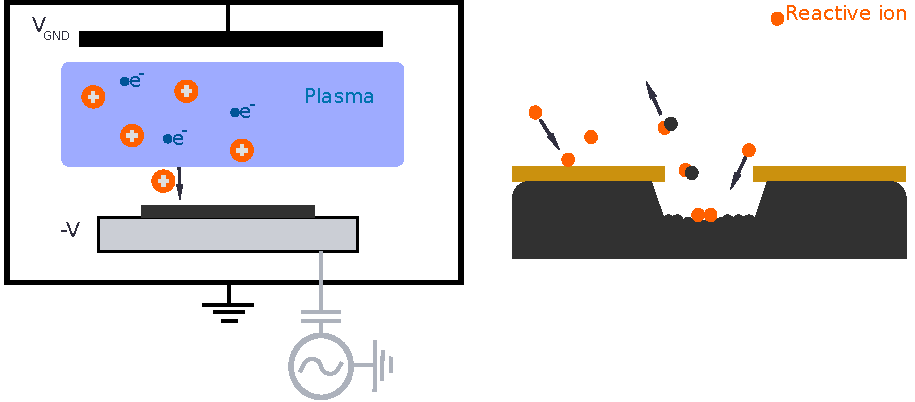
\includegraphics[width=1.0\textwidth]{images/RIE.pdf}
    \caption{Operation principle of a capacitively coupled RIE system and the anisotropic etching profile.}
    \label{fig:RIE}
\end{figure}


This is only the basic principle of RIE. Multiple parameters such as, RF-power, DC-bias, pressure, gas flow rate and temperature all affect the etching process. All of these need to be tuned, to achieve good anisotropy, correct etch rate, and selectivity. The etch chemistry is defined by the gas chosen. Correct selectivity between mask and substrate, and volatile product formation is critical. There are already many well known recipes for RIE, in example, fluoride based gases (like $\mathrm{SF_6}$) are used for silicon etching. For silicon dioxide, $\mathrm{CHF_3}$ is a common choice because of its selectivity to silicon. It will produce $\mathrm{SiF_4}$ and $\mathrm{CO_2}$ as products which are both volatile (boiling points $\SI{-90}{\celsius}$, $\SI{-56}{\celsius}$).  \cite{franssila2010introduction}
RIE equipment can be used for cleaning or activating wafers. An oxygen ($\mathrm{O_2}$) treatment can be used to oxidize and remove organic contamination, which can be residues from organic solvents (acetone) or resists. An $\mathrm{O_2}$ plasma treatment will create a silicon oxide surface on the surface of silicon, or in our case, glass. A following rinse in DI water will then grant a hydroxylated surface. Even wafer bonding has been demonstrated with plasma activated surfaces \cite{plach2013mechanisms,poulsen2003towards}


\subsection{Glass bonding}
\label{sec:xx6}
Wafer bonding is often used in microfabrication when two or more wafers need to be merged together. Bonding mechanisms between two materials can be anodic, direct, or adhesive.  In our case the cover glass needs to be bonded to the patterned glass to form complete channels. Tn the case of two glass surfaces, direct bonding can be applied. Activating both to-be-bonded surfaces will cause the surfaces to be saturated with hydroxyl groups. Bringing the surfaces close enough (under $\SI{2}{\nano \metre}$) van der Waals bonding will occur (Figure \ref{fig:TADB}) \cite{iliescu2012practical}.  The bond strength depends on surface roughness; the number of bonds depends on the area where distance is short enough between the wafers. This weak bonding can be increased significantly by annealing. High temperatures cause the water molecules to diffuse from the surface into the bulk material, thus allowing covalent bonding between the surfaces;
\newline 
\centerline{$\mathrm{Si-OH + HO-Si \rightarrow \;\; Si-O-Si} $}
\newline
The formed bond is between the wafers will be as strong as the bulk material itself, hence Thermal Assisted Direct Bonding (TADB). Bonding glass to glass has also the benefit of both surfaces having the same thermal coefficients, thus stress can be avoided. \cite{franssila2010introduction}

\begin{figure}[h]
    \centering
    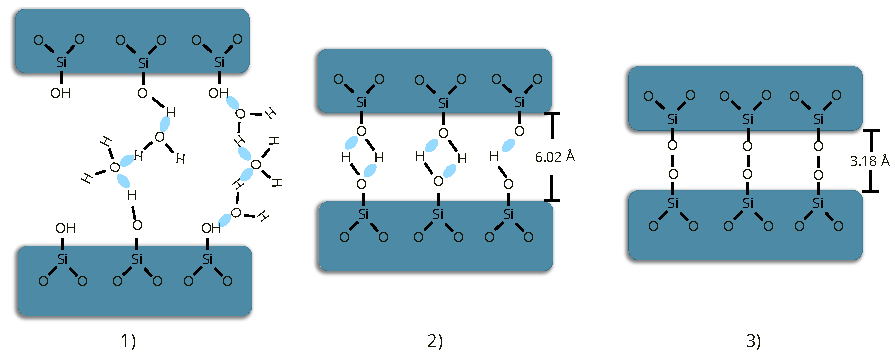
\includegraphics[width=1.0\textwidth]{images/TADB.pdf}
    \caption{Stages occouring during direct bonding. 1) At room temperature (RT)$-110 \celsius$. 2) At $110 \celsius - 150\celsius$ water molecules diffuse away. At $150 \celsius - 800\celsius$ the hydroxyl groups in in close contact form covalent bonds. Adapted from John Wiley and Sons \cite{tong1999semiconductor}.}
    \label{fig:TADB}
\end{figure}


The bonding procedure consists of substrate cleaning and activation, room temperature bonding, and annealing under slight pressure. The cleaning procedure is extremely delicate because any contaminant will increase the distance between the surfaces and will lead to unsuccessful bonding. The temperature and pressure for TADB needs to be optimised for good bonding strength. The optimised temperature and pressure for Soda-lime glass bonding is determined to be $\SI{580}{\celsius}$, $\SI{28}{\kilo \pascal}$ \cite{chen2009thermal}. To achieve the correct pressure, small weights can be used on top of the substrate while in the furnace.

\section{Fabrication}
\label{sec:fabrication}

The aim was to produce $\SI{30}{\micro \metre}$ deep channels cost and time efficiency. The channels would also need to be smooth and defect free to prevent leaking. To have an efficient development process, chips were manufactured in batches of four to account for possible mistakes. At first, every fabrication step was tested on non-drilled chips, to perfect the process. The aim was to reproduce the process developed in Dr. Ján Borovský’s thesis on sorting of carbon nanotubes, which was the further developed by Suha Öcal to better suit for deeper etching \cite{borovsky,suha}. The fabrication steps required a dust free environment, hence they were performed in an ISO5 clean room. As substrate, Menzel-Gläser $20\times20\times1 \milli \metre^{3}$ microscope coverslips consisting of soda-lime glass were used. The chips were drilled with \textcolor{red}{[LASER]} to form the inlets and outlets. 
\newline
\newline
\textbf{Instrumentation:}

For evaporation, Balzers Baltec BAE 250 e-beam evaporator was used at a vacuum of (\numrange[range-phrase = -]{1}{2})$\;\cdot 10^{-5} \milli \torr$. As SEM for EBL, Raith e-Line was used together with its proprietary software \textcolor{red}{[????]}, which includes a CAD tool for layout designing.  For plasma cleaning, activating and etching (RIE) Oxford Instruments Plasmalab80Plus was used. Imaging of the samples was done by Olympus BX51M   together with Q Imaging MicroPublisher 5.0 RTV camera. Chemical processes were conducted in fume hoods and spin-coating in laminar flow-hoods. To determine surface roughness and channel depth a KLA Tencor P-15 profilometer was used. A Laurell WS-650MZ-23NPPB spinner was used for spin coating. The chemicals used are presented in Appendix \ref{sec:chemicals}.

\subsection{Design}
\label{sec:xxx1}
The chip layout was designed using the electron microscopes own software (\textcolor{red}{Raith e-Line 150 ver. 5.0???}). There were two main considerations for the design; The important features required for the chip operation needed to be implemented and it needed to be simplistic allowing a low exposure time. When developing the fabrication steps, it is important to that all the features required can be produced once the fabrication steps are mastered. The most important features were the channels with depth ranging between $(2-40) \mathrm{\micro \metre}$, width of $(10-120) \mathrm{\micro \metre}$ and the manufacture of electrodes close as possible to the channels. E-beam was chosen as the lithography method for development to allow fast changes in design if necessary, without the need to create new masks as in photolithography. E-beam exposure time increases with area exposed, which had to be minimized for efficient development. 
\begin{figure}[h]
    \centering
    \begin{subfigure}[ht]{0.65\textwidth}
        \centering
        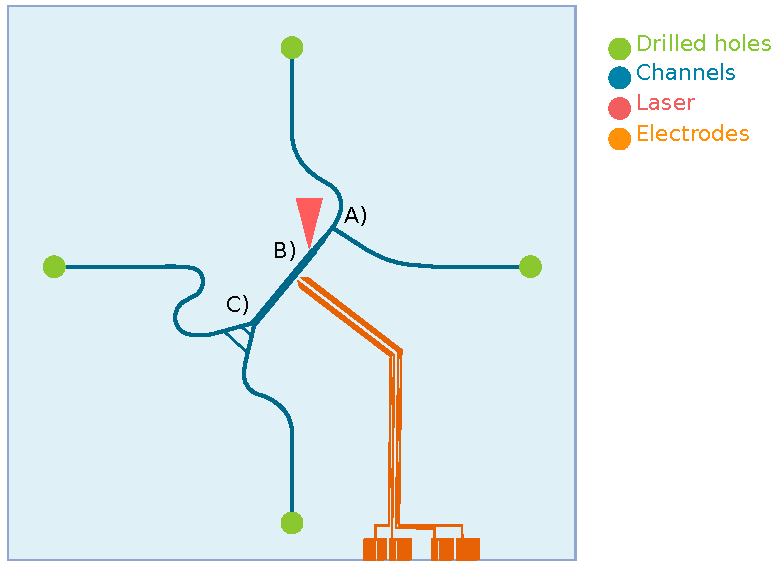
\includegraphics[width=\linewidth]{images/chip_design.pdf} 
        \caption{Chip layout.} \label{fig:design1}
    \end{subfigure}
    \hfill
    \begin{subfigure}[ht]{0.33\textwidth}
        \centering
        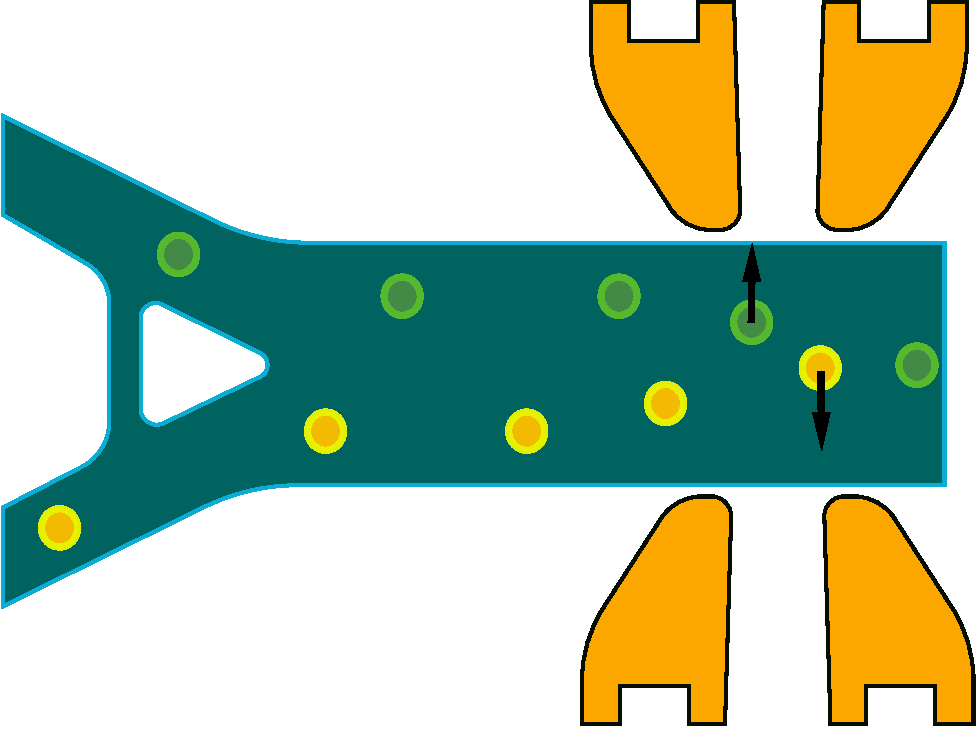
\includegraphics[width=\linewidth]{images/Separation.pdf} 
        \caption{Deflection of cells to different lanes} \label{fig:flow1}
    \end{subfigure}
    \caption{The design for the layout of the microfluidic chip.} \label{fig:design_flow}
\end{figure}  

The three most important areas of the channel layout are visualised in Figure \ref{fig:design1}. A) The channels from the two inlets meet at a T-crossing. It allows droplet formation, if droplet-based sorting is to be used, or flow control. If cells are inserted from one of the inlets, the space/medium between the cells can be altered by tuning the second inlet pressure. This flow adds medium in between the cells thus increasing the distance between them. B) Is a narrow channel confining the cells for analysis then expanding into a long and wide channel. In the wider part the flow would slow down due to higher volume and the electrodes placed next to the channel would push or pull the cells based on their fluorescence. Assuming a laminar flow, the cells would then take the correct “lane” in the wide channel to be then sorted. C) At the Y-junction the cells would go left or right depending on their “lane” to be collected or to become waste (Figure \ref{fig:flow1}). The junction would also require small channels where cells don’t fit across to stabilize pressure. A cell going in right channel would then increase the drag on the fluid thus causing the left channel to be more favourable for the next incoming cell independent of its lane.

The layout was designed for a chip of $20 \times 20 \; \milli \metre$, where the two inlets and two outlets were each $\SI{7}{\milli \metre}$ from the chips centre point (Figure \ref{fig:design1}).  The channels were designed to curve smoothly without rough edges and shapes to uphold laminar flow and reduce clogging. The channel width was $\SI{30}{\micro \metre}$ for the transport of cells and $\SI{5}{\micro \metre}$ for the pressure stabilizing channels. At the electrodes, the channel width was up to $\SI{50}{\micro \metre}$ to allow proper flow lanes for the cells. The design needed to accommodate for isotropic etching, meaning the channels were always wider than the exposed width. Knowing the correct width was critical in placing the electrodes close as possible. Concerning the length, the straight part in front of the electrodes needs to be long enough for the spectroscopy and the separation to take place. The inlet channels before the T-junction and the outlet channels after the Y-junction were designed to have matching lengths. Especially for the outlets it is essential because otherwise there would be a pressure difference that would make one channel more favourable for the flow.

The design for the electrodes were reproduced for Borovský’s thesis \cite{borovsky}. The tip shape originated from a paper, where the electric fields were simulated to produce an ideal electric field for contactless DEP \cite{leman_droplet-based_2015}. The electrodes consisted of a half loop having contact pads at the end for allowing the test whether they were functional. The contact pads were split into vertical lines to reduce the exposure area and thus time significantly. The final optimal design would include uniform contact pads and four electrodes. If Same frequency pDEP or nDEP is to be achieved there need to be electrodes on both sides of the channel. For the process development only two electrodes were manufactured. 


\subsection{Overview of the process}
\label{sec:xxx2}

The realization of the microfluidic chip was performed with conventional micro-fabrication-methods. Varying steps and methods were tried through trial and error until success. The fabrication steps for a successful chip are shown in Figure \ref{fig:processFULL}.
1) Drilled Soda Lime-glass microscope coverslips are used as substrate. The glass chip is first cleaned and treated with Piranha-solution prior to evaporation. 2) Using E-beam evaporation, a of $\SI{100}{\nano \metre}$ Cr thin film is evaporated to act as an etch mask. Next, PMMA of about $\SI{250}{\nano \metre}$ is spun before e-beam exposure. 3) The electrode design is then exposed and developed. 4) The Cr-mask etched followed by a dip into HF-HCl (10:1) solution to etch shallow grooves for the electrodes. After etching, a RIE $\mathrm{O_2}$ etch was used to activate the glass and clean PMMA residue from electrode channels. 5) Electrodes are then evaporated; a metal sandwich of $\SI{10}{\nano \metre}$ Ti +$\SI{50}{\nano \metre}$ Au +$\SI{10}{\nano \metre}$ Ti +$\SI{100}{\nano \metre}$ $\mathrm{SiO}_2$). 6) Lift-off is then carried out and the Cr-mask etched away. 7) A tougher RIE O2 treatment is used to activate the glass surface and $\SI{50}{\nano \metre}$ Cr + $(150 + 150) \,\nano \metre$ Au is evaporated in an $45^{\circ}$ angle while the wafer is rotated ensuring deposition to the walls of the trenches. 8) Now $\SI{2.2}{\micro \metre}$ of PMMA is spun to cover the shallow channels of the electrodes completely. 9) Alignment, exposure, and development of the Channels-layout is performed. 10) The Au and Cr masks are etched followed by a 55s HF-HCl etch of the channels. After removing the e-beam resist the gold mask is removed by etching the underlining Cr. 11) Finally, the chip and its cover are cleaned and activated in Piranha so can be bonded. The bonding is performed in a furnace at $\SI{85}{\celsius}$ for 2h. The bonded chip is then treated with a RIE oxide etch to reveal the electrode pads for soldering and the chip is ready.





\textcolor{red}{figureas at wrong page for now, NEEDS a fix}
%Make numbers in figures go 1,2,3 instead of a b c
\renewcommand{\thesubfigure}{\arabic{subfigure}}

\begin{figure}
    \centering
    \begin{subfigure}[hb]{0.48\textwidth}
        \centering
        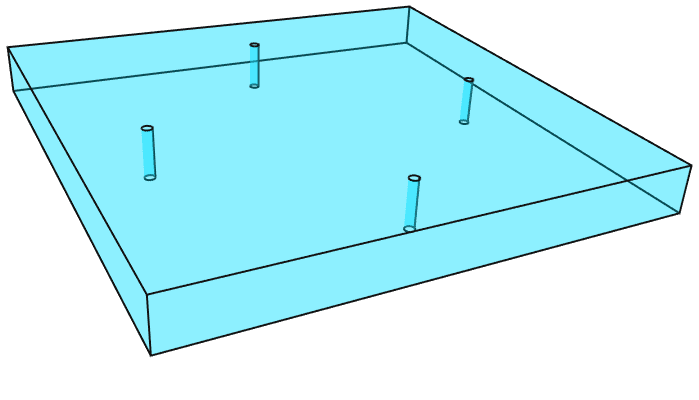
\includegraphics[width=\linewidth]{steps/1.Drilled.png} 
        \caption{Drilled Soda-lime glass chip} \label{fig:process1}
    \end{subfigure}
    \hfill
    \begin{subfigure}[hb]{0.48\textwidth}
        \centering
        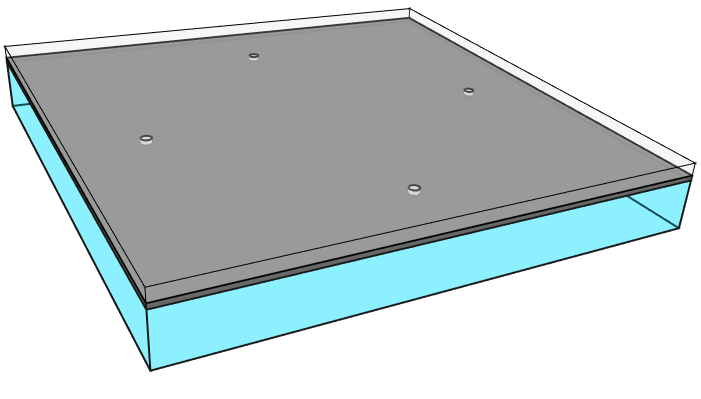
\includegraphics[width=\linewidth]{steps/2.Cr-Pmma.png} 
        \caption{$\SI{100}{\nano \metre}$ Cr + $\SI{250}{\nano \metre}$ PMMA} \label{fig:process2}
    \end{subfigure}
    
    \begin{subfigure}[b]{0.48\textwidth}
        \centering
        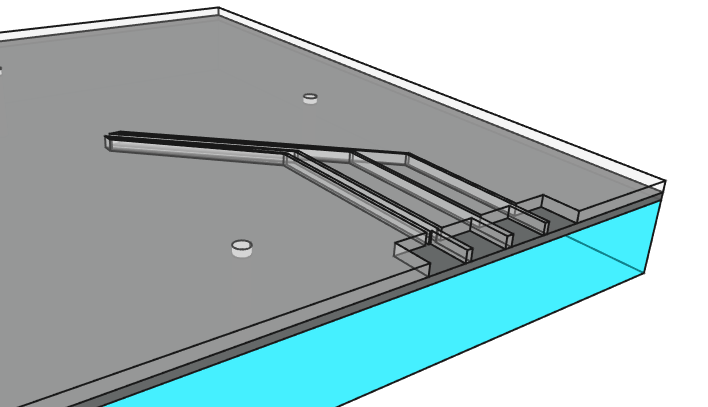
\includegraphics[width=\linewidth]{steps/3.Developed.bmp.png} 
        \caption{PMMA developed} \label{fig:process3}
    \end{subfigure}
    \hfill
    \begin{subfigure}[b]{0.48\textwidth}
        \centering
        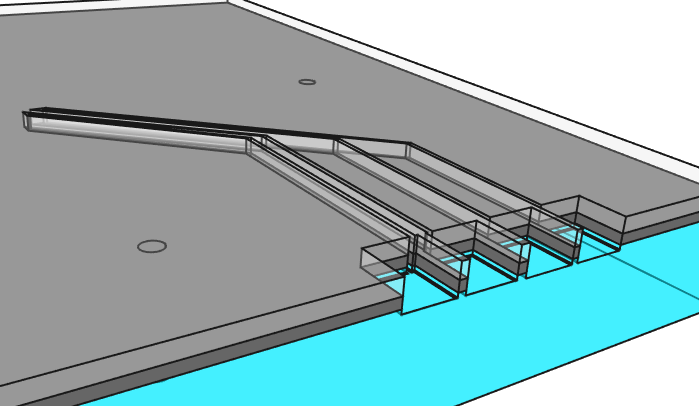
\includegraphics[width=\linewidth]{steps/4.Etched.png} 
        \caption{Cr-mask and Glass etched} \label{fig:process4}
    \end{subfigure}
    
    \begin{subfigure}[b]{0.48\textwidth}
        \centering
        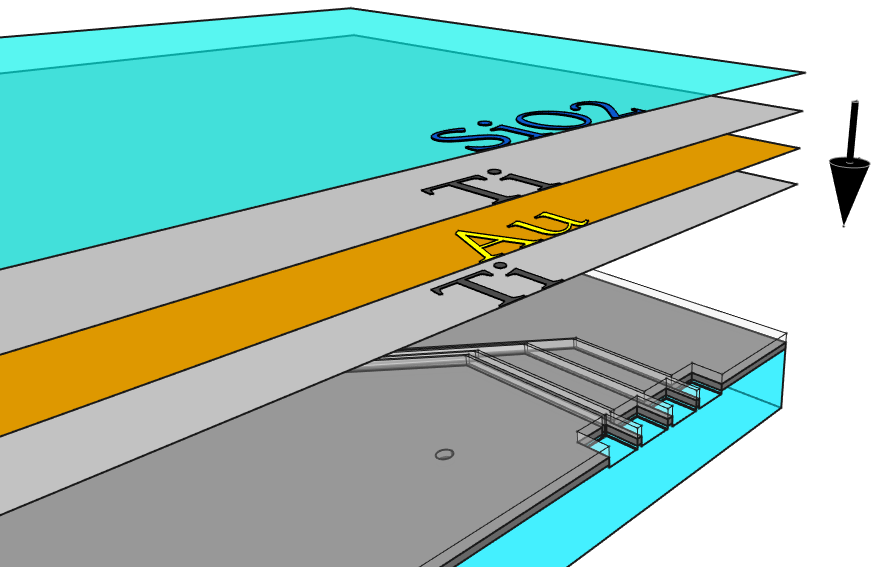
\includegraphics[width=\linewidth]{steps/5.-evap-Elec.png} 
        \caption{Electrodes deposited ($\SI{10}{\nano \metre}$ Ti + $\SI{50}{\nano \metre}$ Au + $\SI{10}{\nano \metre}$ Ti + $\SI{100}{\nano \metre}$ $\mathrm{SiO}_2$) } \label{fig:process5}
    \end{subfigure}
    \hfill
    \begin{subfigure}[b]{0.48\textwidth}
        \centering
        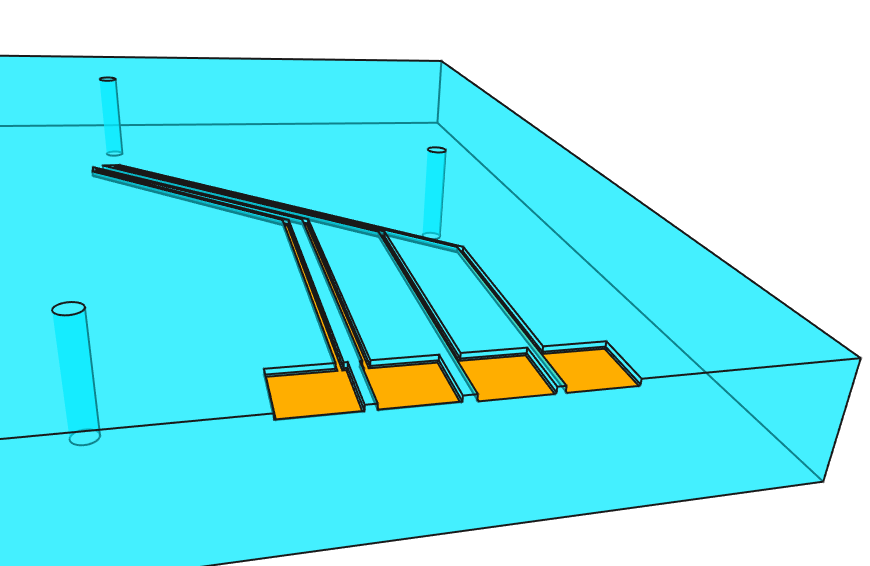
\includegraphics[width=\linewidth]{steps/6.-lift_off.png} 
        \caption{Lift-off} \label{fig:process6}
    \end{subfigure}
    
    \begin{subfigure}[b]{0.48\textwidth}
        \centering
        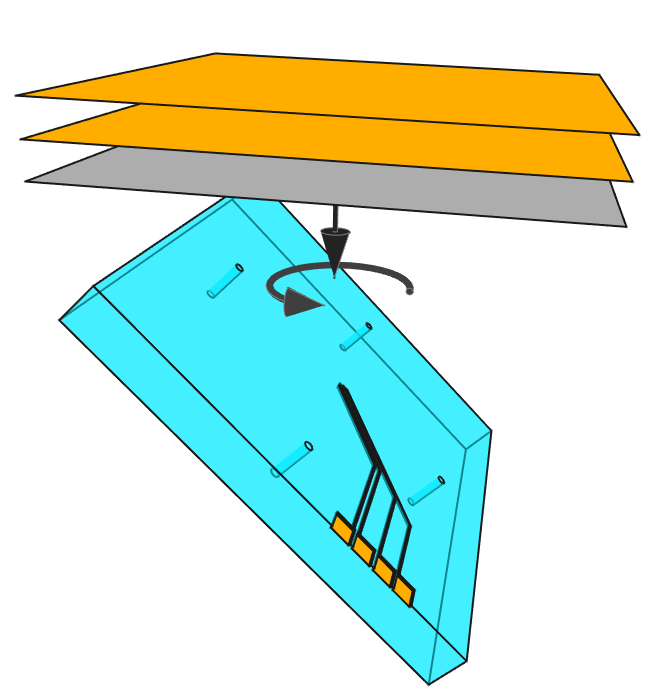
\includegraphics[width=\linewidth]{steps/7.evap_mask.png} 
        \caption{$\SI{50}{\nano \metre}$ Cr + $(150 + 150) \,\nano \metre$ Au deposited at $45^{\circ}$ angle on a spinning wafer} \label{fig:process7}
    \end{subfigure}
    \hfill
    \begin{subfigure}[b]{0.48\textwidth}
        \centering
        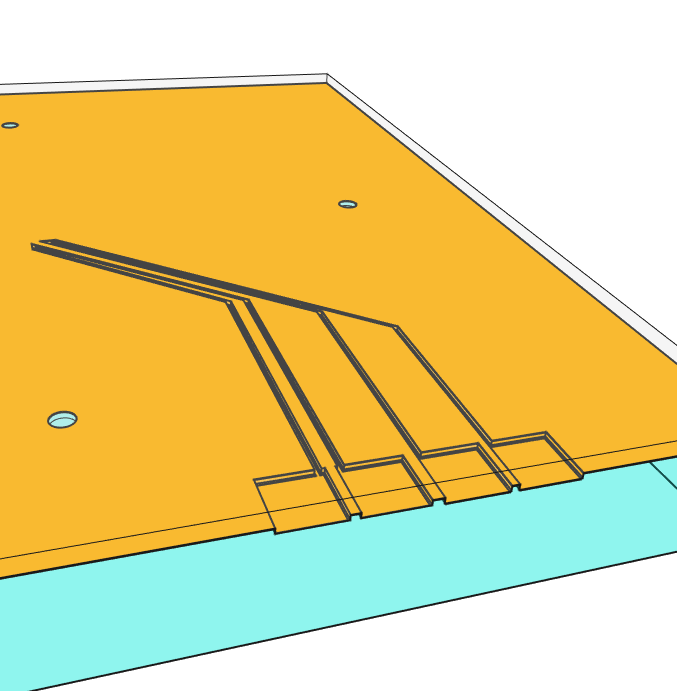
\includegraphics[width=\linewidth]{steps/8.pmma-thick.png} 
        \caption{$\SI{2.2}{\micro \metre}$ PMMA} \label{fig:process8}
    \end{subfigure}
\end{figure}  

%\captionsetup[subfigure]{labelformat=empty}
\begin{figure}\ContinuedFloat
    \centering    
    \begin{subfigure}[t]{0.48\textwidth}
        \centering
        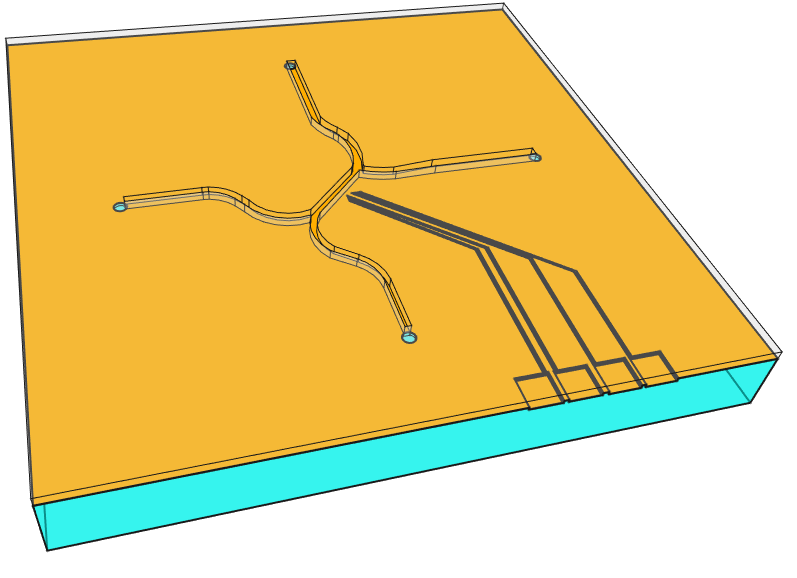
\includegraphics[width=\linewidth]{steps/9.developed2.png} 
        \caption{ Development} \label{fig:process9}
    \end{subfigure}
    \hfill
    \begin{subfigure}[t]{0.48\textwidth}
        \centering
        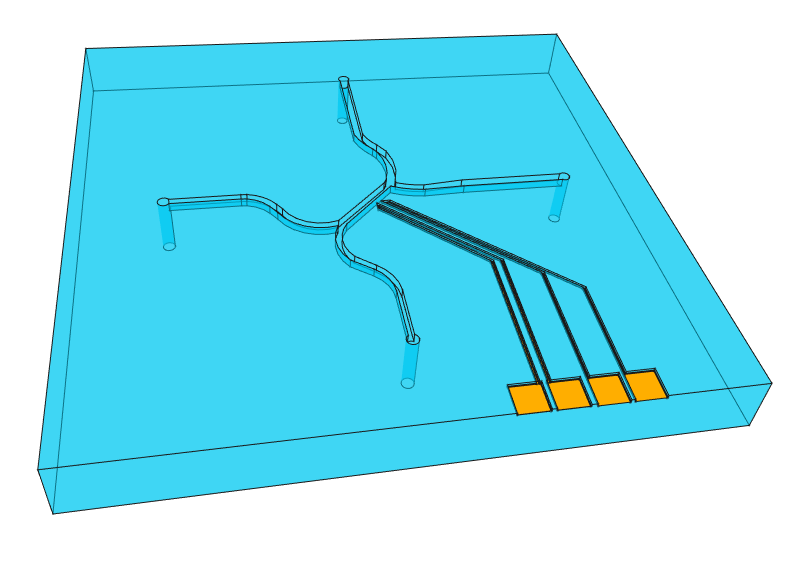
\includegraphics[width=\linewidth]{steps/10.etched.png} 
        \caption{Liftoff by etching Cr} \label{fig:process10}
    \end{subfigure}
    
    \vspace{1cm}
    \begin{subfigure}[t]{\textwidth}
    \centering
        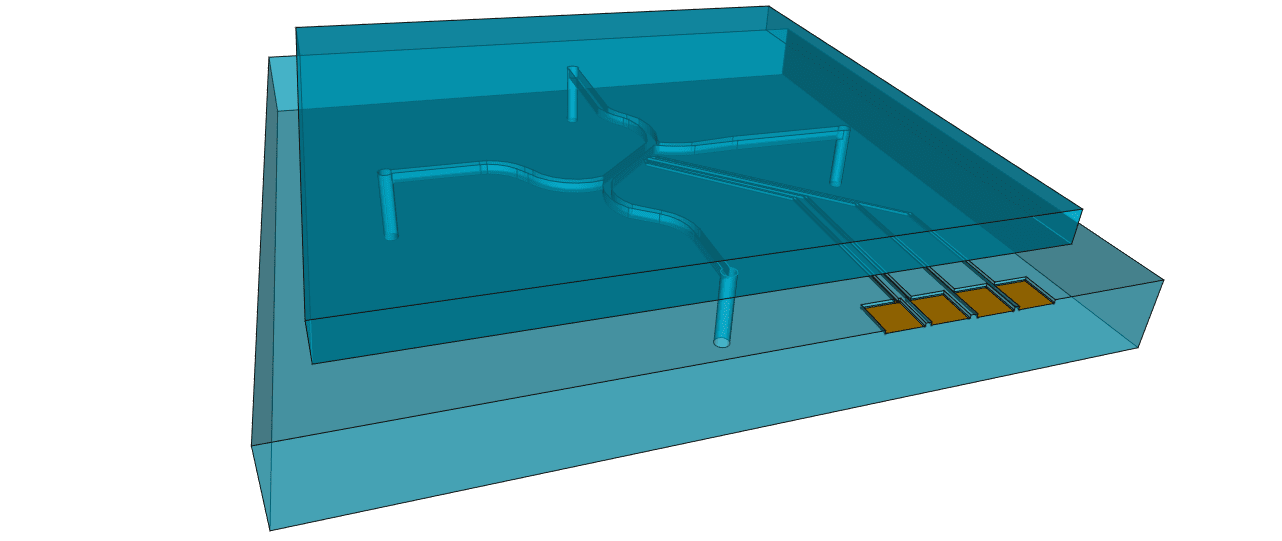
\includegraphics[width=\linewidth]{steps/11.Finished.png} 
        \caption{Thermally bonded cover} \label{fig:process11}
    \end{subfigure}
    \caption{The fabrication steps for a functional microfluidic chip} \label{fig:processFULL}
\end{figure}

\subsection{Channels}
\label{sec:xxx3}

\subsubsection{Initial fabrication}

For etch mask deposition, the chips needed to be contaminant free. Glass residue and leftover protective tape from drilling were removed by mechanical scrubbing and hot acetone. The chips were then rinsed with IPA and dried with $\mathrm{N_2}$ gun. 
To clean organic residue from Acetone+IPA and to Activate the glass surface, a piranha clean was performed. The piranha solution made from 3:1 Sulphuric acid and hydrogen peroxide and kept at $100 \celsius$ for 40 minutes. When done, the chips were dipped into $\mathrm{dH_2 O}$ for rinsing any Piranha residues. A layer of $\SI{50}{\nano \metre}$ Cr and $\SI{200}{\nano \metre}$ Au was then evaporated at a speed of $\SI{1.0}{\angstrom \per \sec}$.
After evaporation, PMMA 950K A4 was spin coated at 3000 rpm and prebaked at 160$\celsius$ for 2 min. A test pattern layout, containing traps and channel intersections was then exposed using EBL with $\SI{215}{\micro \coulomb \per \centi \metre^{2}}$, developed in MIBK:IPA for 45s and stopped in IPA. The resist was then hard baked at $200 \celsius$ for 2h on a hot plate. The gold layer was then etched using Gold etchant (Appendix \ref{sec:chemicals}) for 15s and Cr using Nichrome etchant (Appendix \ref{sec:chemicals}) for 10s.  The glass was then etched with 48\percent HF (Appendix \ref{sec:chemicals}) for 1 min. Finally, the resist was removed with acetone and both Cr and Au masks etched away completely within their corresponding etchants.

The result was poor and barely enough for an operational chip. The channel surfaces were rough, and the chip was filled with pinholes (Figure \ref{fig:pinhole}). The mask was also in poor condition, containing a lot of pinholes and occasional blister like features underneath. The adhesion of the mask to the substrate was weak which was obvious from mask detachment during sonification. Fixing these issues was not trivial, because the process consisted of many fabrication steps and it was unknown what was the exact cause of these defects. It also took time to master basic cleanroom procedures like precise tweezer handling to minimize mechanically caused defects to the chips. 

%Make numbers in figures go 1,2,3 instead of a b c
\renewcommand{\thesubfigure}{\arabic{subfigure}}

\begin{figure}[!h]
    \centering    
    \begin{subfigure}{0.48\textwidth}
        \centering
        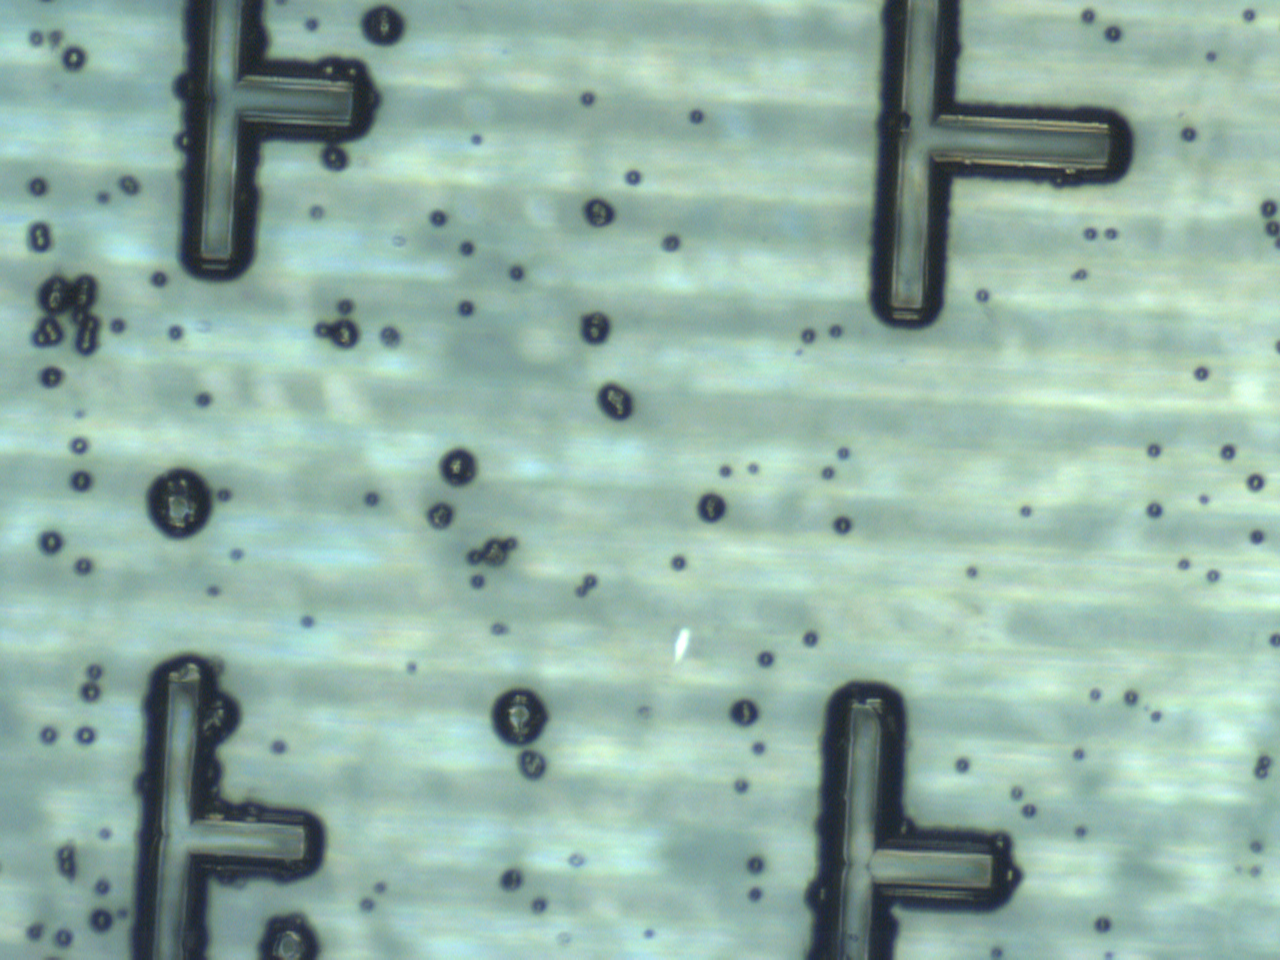
\includegraphics[width=\linewidth]{optical/pinholes1.png} 
        \caption{Pinholes} \label{fig:pinhole1}
    \end{subfigure}
    \hfill
    \begin{subfigure}{0.48\textwidth}
        \centering
        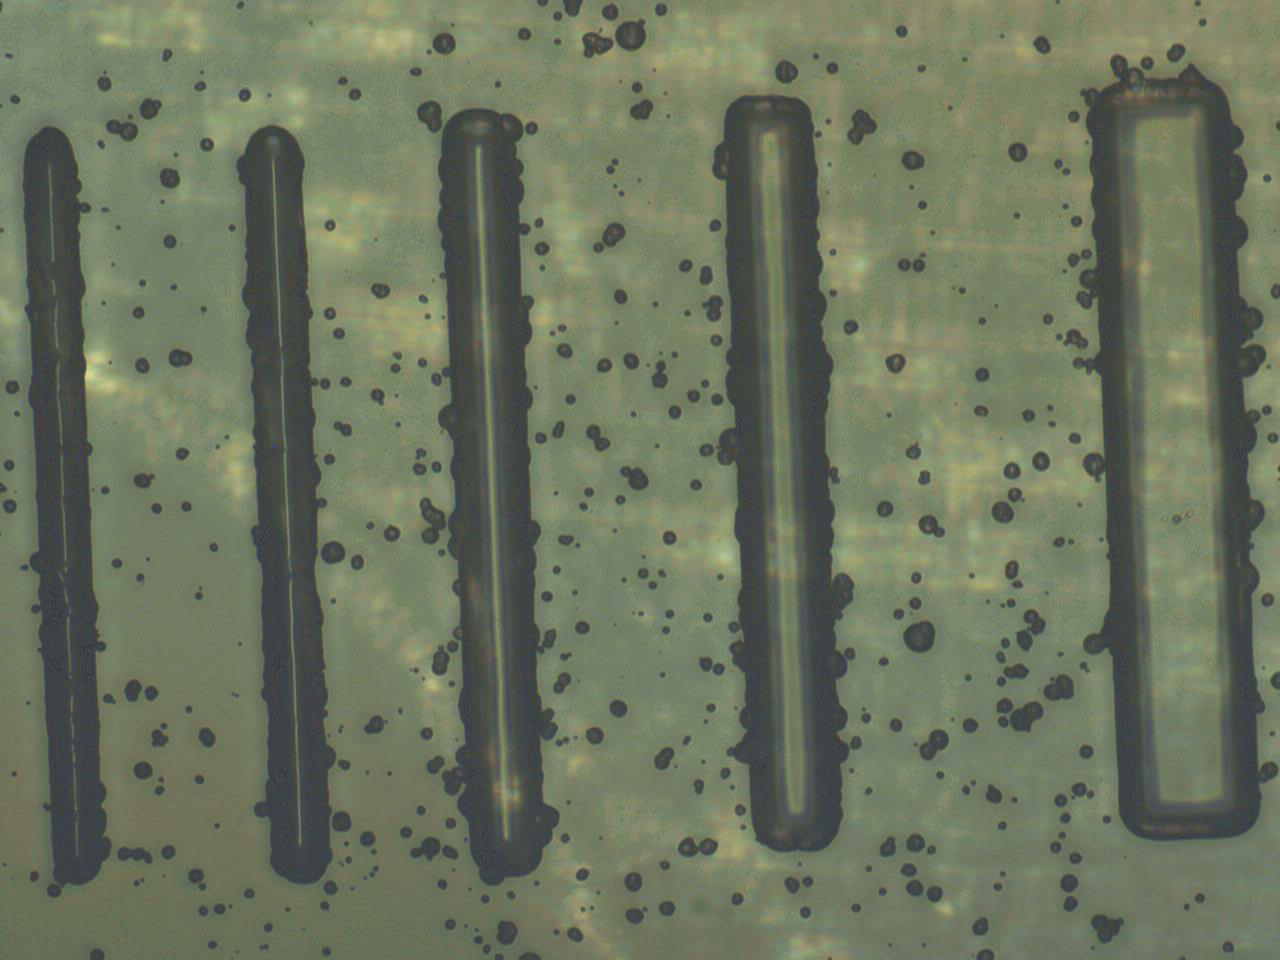
\includegraphics[width=\linewidth]{optical/pinholes2.png} 
        \caption{Pinholes} \label{fig:pinhole2}
    \end{subfigure}
    
    \vspace{1cm}
    \begin{subfigure}{\textwidth}
    \centering
        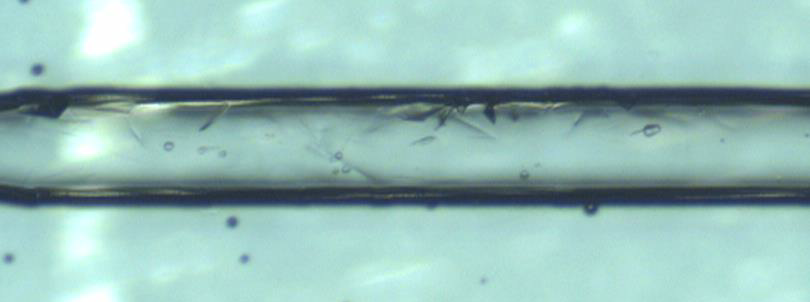
\includegraphics[width=\linewidth]{optical/roughness2.png} 
        \caption{Channel roughness} \label{fig:roughness}
    \end{subfigure}
    \caption{The defects present in the initial fabrication.} \label{fig:pinhole}
\end{figure}



\subsubsection{Troubleshooting}

\begin{flushleft}\textbf{Channel roughness} \end{flushleft}
The channel roughness was addressed first. It seemed to have a sort of randomness, some chips having smoother channels than others. Although, it did appear more consistently in thinner channels ($\SI{5}{\micro \metre}$ in design) and was almost non-existent in wide areas (over $\SI{30}{\micro \metre}$ in design). After a thorough literature search, it was obvious that soda-lime glass forms insoluble products with HF. The impurities (CaO, $\mathrm{Al_2 O_3}$, MgO) present in soda lime will form precipitates \cite{lin2001fast,iliescu2005characterization}:
\newline
\centerline{$\mathrm{ CaO \rightarrow CaF_2,\; MgO \rightarrow MgF, \; Al_2 O_3 \rightarrow AlF_3}$}
\newline
By adding HCl into the etchant, these products can be made soluble:
\newline
\centerline{$\mathrm{CaF_2 \rightarrow CaCl_2, \; MgF \rightarrow MgCl_2, \; AlF_3 \rightarrow AlCl_3}$}

Iliescu et al. (2005) found the optimal ratio for HF:HCl to be 10:1 concerning surface roughness and etch rate \cite{iliescu2005characterization}. Due to practical convenience (beaker size) $\SI{48}{\percent}$ HF was mixed with $\SI{37}{\percent}$ HCl (Appendix \ref{sec:chemicals}) in a ratio 9:1 ($\SI{18}{\milli \litre}:\SI{2}{\milli \litre}$). This caused a significant improvement in surface roughness. These roughness defects were still present in the thinner channels and at the outlines of the channels that were isotopically etched under the mask. This is probably a result from fresh etchant not being able to reach small corners and areas as efficiently, thus the mixing of the insoluble products with the bulk solution was slowed. Gentle mixing was applied during HF-etching to overcome the problem. The gentle wiggling of the chip during etching did yield better results but to totally overcome the problem sonication would be required. Sonication was not applied due to safety reasons of the toxic HF.


\begin{flushleft}\textbf{Mask quality} \end{flushleft}
To fix the mask quality to an acceptable level, almost every fabrication step had to be slightly improved. The two main reasons for bad mask quality were contaminated substrate surface and poor evaporation quality. To improve the cleanliness of the surface, the scrubbing and sonication in acetone -step was repeated multiple times. Sonication and rinse in IPA were also applied. The chips were the checked against light to see whether all visible contaminants have been removed. The chips were put in a flat beaker in $\mathrm{dH_2 O}$ to avoid any contamination from ambient air while transporting them between fabrication steps. 
To improve the film adhesion activation step was altered. Different concentrations (2-5):1 were tried with varying activation times (30 min $\-$ 1h), but they did not alter the outcome on an observable level. The piranha treatment was altered to last 30 min, then a thorough rinse (over 30 s) in $\mathrm{dH_2 O}$ and putting it back to the piranha (cool) solution for 10 min. The chips were then again thoroughly rinsed and put in $\mathrm{dH_2 O}$. This was done to increase hydroxyl groups on the surface and to rinse any contaminants. Careless cleaning of piranha residues from the chip leads to disastrous results (Figure \ref{fig:piranjaaa}). Prior to evaporation the chips were put on a hotplate at $\SI{130}{\celsius}$ for 2 min to evaporate all moisture. Higher temperatures were avoided to avoid the desorption of the carboxyl groups.

\begin{figure}[h]
    \centering
    \begin{subfigure}[ht]{0.48\textwidth}
        \centering
        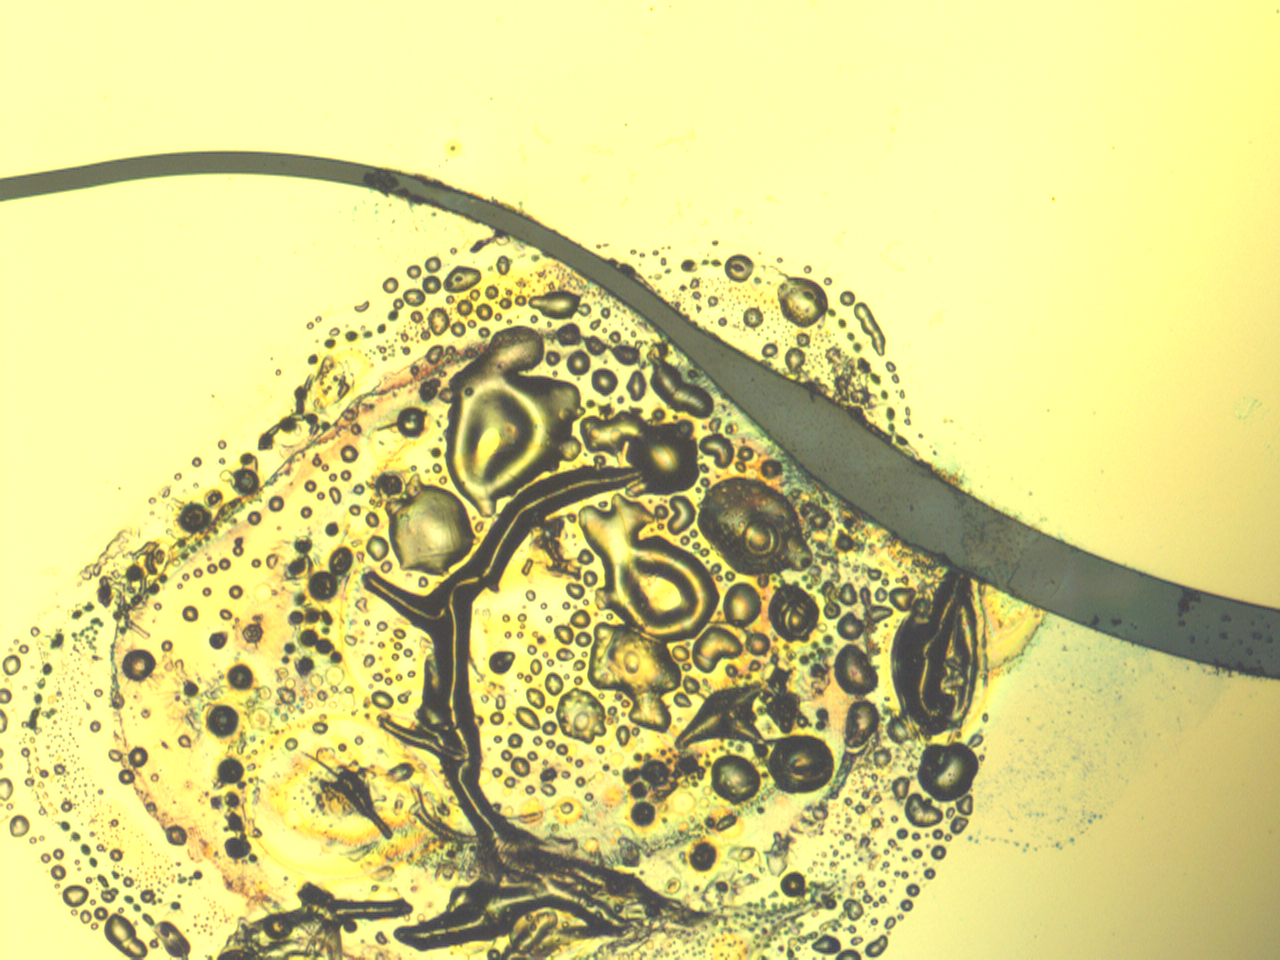
\includegraphics[width=\linewidth]{optical/bad_piranha.png} 
        \caption{} \label{fig:piranjaaa}
    \end{subfigure}
    \hfill
    \begin{subfigure}[ht]{0.48\textwidth}
        \centering
        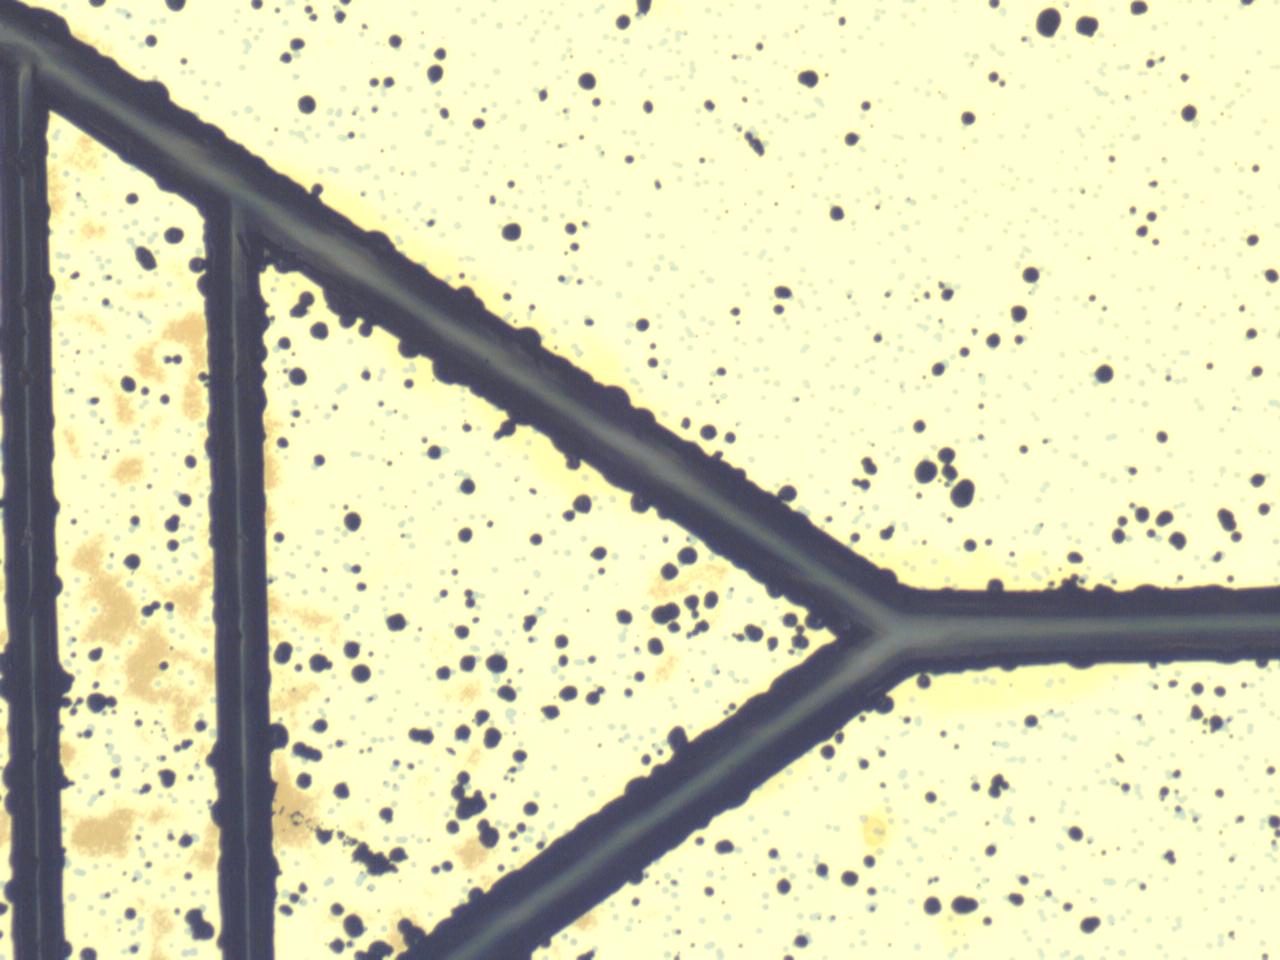
\includegraphics[width=\linewidth]{optical/faultyevap.png} 
        \caption{} \label{fig:faultyy}
    \end{subfigure}
    \caption{1) Piranha residue under mask layer. Only visible after evaporation. 2) Bad mask quality due to failed evaporation.} \label{fig:bad_piranha}
\end{figure}  

A set of challenges were faced with the evaporator. Electrical conductivity problems were randomly present causing difficulties on setting a constant evaporation speed (Figure \ref{fig:faultyy}). Conductivity problems also caused current spikes that hit the crucible, thus evaporating crucible material and causing film contamination. The evaporator being under constant use, various evaporation materials accumulated around the crucible. By distorting the magnetic field, this led to the electrons missing the target material and hitting the crucible. Cleaning of the evaporator and sonication the target material and the crucible in IPA before evaporation, had a noticeable positive effect. The target Cr was also changed to fresh unoxidized pellets and there-on kept in $\mathrm{N_2}$ atmosphere cupboard to avoid oxidation. 

Consequently, the number of pinholes were reduced but not completely eliminated. Multiple researches suggest having a double layer of gold to reduce pinholes \cite{iliescu2008wet,Hgglund2013CharacterizationOM,bu2004new}. The idea is that when pinholes are generated from contamination particles or the stress of the film, they will be generated randomly. Depositing a second layer on top, that will also have defects randomly, the second layer would mostly cover the pinholes generated in the first layer. Between the depositions the film would be cooled and the defects generated due to tensile stress (Figure \ref{fig:multilayer_mask}). 
Combinations of $\SI{70}{\nano \metre} + \SI{70}{\nano \metre} + \SI{70}{\nano \metre}$, $\SI{150}{\nano \metre}+ \SI{150}{\nano \metre}$ and $\SI{200}{\nano \metre} + \SI{100}{\nano \metre}$ Au layers were tried. The triple $\SI{70}{\nano \metre}$ layer was weak with a lot of pinholes with the top layer detaching just from sonication. The $\SI{200}{\nano \metre} + \SI{100}{\nano \metre}$  Au with waiting 15 min between depositions yielded a very positive result, thus it was kept as the method for further development.
\begin{figure}[!h]
    \centering    
    \begin{subfigure}{0.40\textwidth}
        \centering
        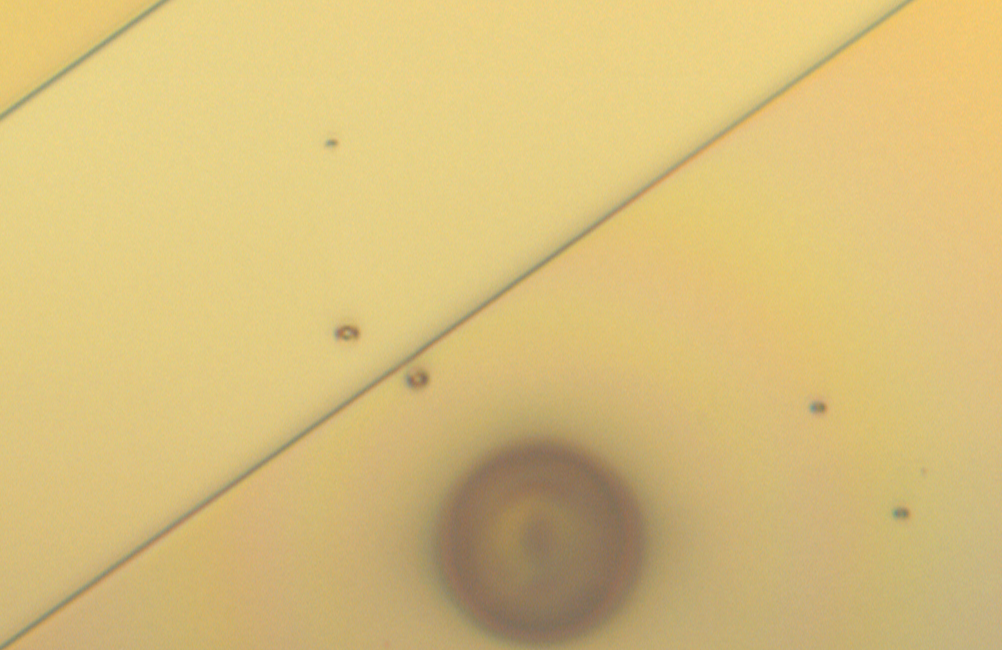
\includegraphics[width=\linewidth]{optical/pinhole00.png} 
        \caption{Pinhole} \label{fig:pinholee}
    \end{subfigure}
    \hfill
    \begin{subfigure}{0.40\textwidth}
        \centering
        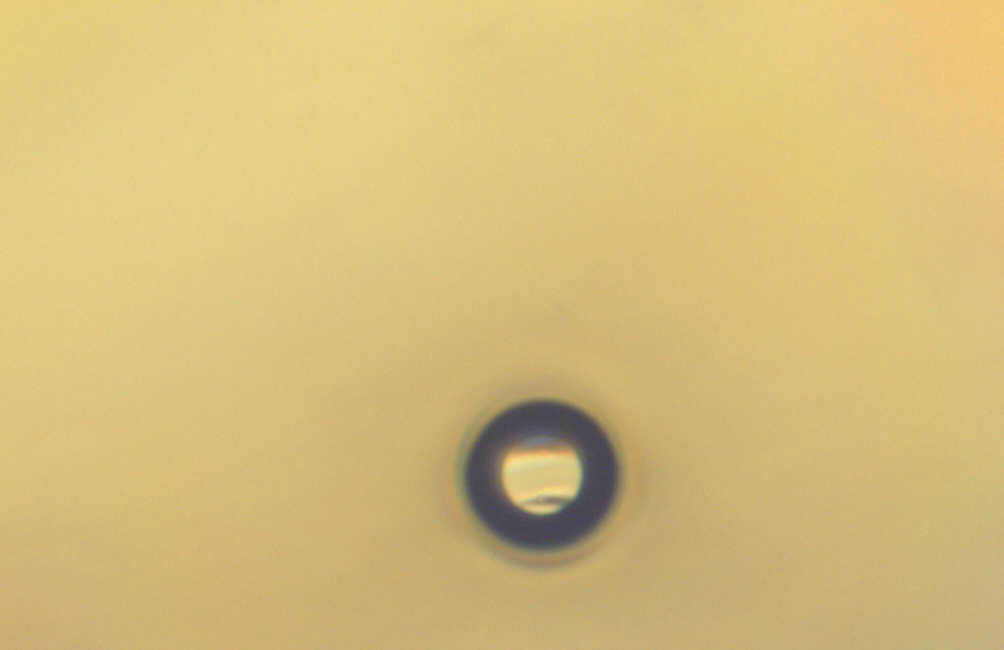
\includegraphics[width=\linewidth]{optical/pinhole01.png} 
        \caption{Focus within pinhole reveals underlining Au layer} \label{fig:pinholeee}
    \end{subfigure}
    
    \vspace{0.2cm}
    \begin{subfigure}{\textwidth}
    \centering
        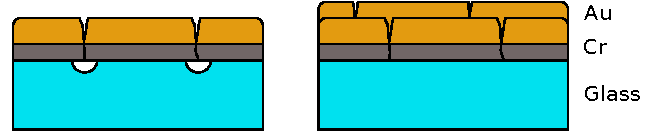
\includegraphics[width=\linewidth]{images/pinhol.pdf} 
        \caption{Double layer Au mask} \label{fig:mask_idea}
    \end{subfigure}
    \caption{The double layered Au mask. When a pinhole is generated in the top layer, the underlining layer can still be intact and protect the sample.} \label{fig:multilayer_mask}
\end{figure}

\begin{flushleft}\textbf{Channels etch} \end{flushleft}
To get the right channel depth the, the etch rate of the HF:HCl solution was determined. The channel depth and profile for various etching times were measured with a Profilometer and it was found to be $\SI{0.55}{\per \sec}$ (Figure \ref{fig:etch_rate}). The isotropy of the etch profile was important in placing the electrodes close to the channels (Figure \ref{fig:sideetch}). The dimensions of the channels were measured using a profilometer; the lateral etch rate averaged to be the same as vertical. 

\begin{figure}[!h]
    \centering
    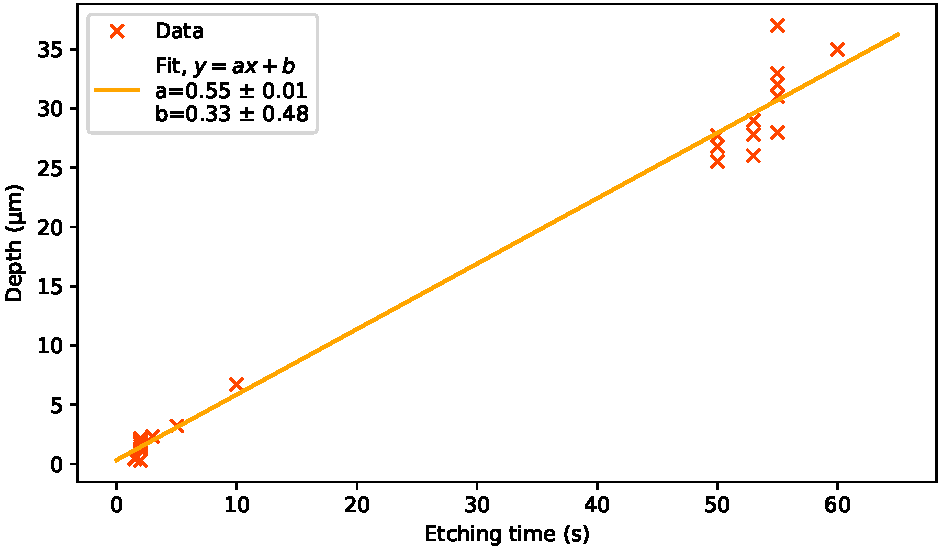
\includegraphics[width=1.0\textwidth]{images/EtchRate.pdf}
    \caption{Etch rate of soda-lime with HF:HCl 10:1. The rate variation is a result of differing channel width. A depth variation up to $\pm 5 \; \micro \metre$ was measured for  channels, wide ones being deeper and vice versa.}
    \label{fig:etch_rate}
\end{figure}

\begin{figure}
    \centering
    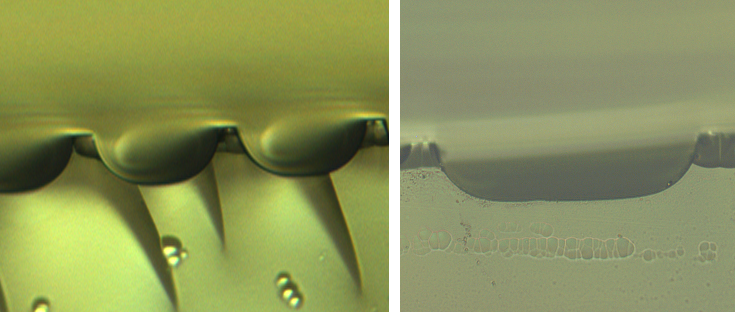
\includegraphics[width=1.0\textwidth]{optical/sideetch.png}
    \caption{The the etch profiles of channels with mask openings of $\SI{10}{\micro \metre}$ (left) and $\SI{50}{\micro \metre}$ (right).}
    \label{fig:sideetch}
\end{figure}

The only requirement for embedding the electrodes within the chip was the electrode-channel being deeper than the electrode thickness (over $\SI{170}{\nano \metre}$). Because high lateral precision was not required, a HF dip was deployed using only PMMA as mask. Dipping times of (1.5s and 10s) with concentrations of HF ($48\percent$ and $20\percent$) were tested, all leading to failure. The resists didn’t get destroyed but it peeled off from the glass. PMMA is resistant to HF but the adhesion layer between glass and PMMA is not. PMMA’s adhesion to glass results from the basic carbonyl groups of PMMA and the acidic silanol (Si-OH) groups on glass surface \cite{tan2008fundamentals}. Either by diffusing through PMMA or between the interface, HF will react with the hydroxyl groups and detach the resist from the glass.

With the absence of a metal mask, the charging of the sample during EBL was solved using a conductive resist on top (Electra 92, Appendix \ref{sec:chemicals}). It is water soluble, meaning that it can be removed before development by dipping in $\mathrm{dH_2O}$ and the hydrophobic PMMA will go unaltered. Due to the failure of this experiment a $\SI{100}{\nano \metre}$ Cr layer was used as etch mask under the PMMA. With hardbaking the resist, the Cr mask proved sufficient for shallow channel etching (etch time 2s).
\newline
\newline
\textcolor{red}{To be cosnidered towards the end!}
(where do I put annealing?,  Batch 8 , not annealed, Trashy channels even with HCl)))

(Evaporation problem > Too high evaporation speed of gold led to chunks flying!)(HAve images but is it important?)

(Batch 11 – STRESS examples)

\subsection{Electrodes}
\label{sec:xxx4}

The electrodes were fabricated to meet the requirements of contactless DEP. This means that they need to be as possible to the microfluidic channels, but avoiding contact. Because of the $\SI{1}{\milli \metre}$ thickens of the chip and the cover glass, the electrodes should be placed in between the glasses. Due to the low surface roughness requirement set by TADB the electrodes cannot be placed between the glasses without immersing them into the glass. For proper bonding, an average surface roughness of $\SI{50}{\nano \metre}$ is allowed \cite{chen2009thermal}. Depositing electrodes (over $\SI{170}{\nano \metre}$ thick) directly on glass surface, would create newton rings and their location next to the channels would cause leakage. 

\begin{flushleft}\textbf{Fabrication} \end{flushleft}
The first decision in electrode fabrication was whether to do it before or after the etching of the main channels. Etching the electrode-channels together with the main channels holds many advantages. Not needing to do a second lithography process (including activation, mask evaporation, exposure etching) would save in time and cost. Reducing the fabrication steps guarantees a higher success rate for a working chip fabrication. Furthermore, etching only once would reduce the amount of pinholes. Simultaneous etching meant that the electrode channels would be the same depth as the main channels. This caused a challenge for protecting the main channels during electrode deposition. The bad step coverage of PMMA leads to unprotected edges (Figure \ref{fig:coverage}) Multiple layers of PMMA were spun as a protective layer, but the steep edges were always left unprotected. A sandwich of PMMA-Cr-PMMA was also tested, but during prebake, the Cr-layer cracked becoming useless. As a last resort, protection of the channels with tape was tried, but it was not suitable for the high precision requirement of the electrode-channel distance.

\textcolor{red}{Decide towards end if needed to be added}
\textcolor{red}{ images of electrode on edge , pmma sandwitch, electrode material through pmma (images/scrubbing)?}



\begin{figure}[h]
    \centering
    \begin{subfigure}[ht]{0.48\textwidth}
        \centering
        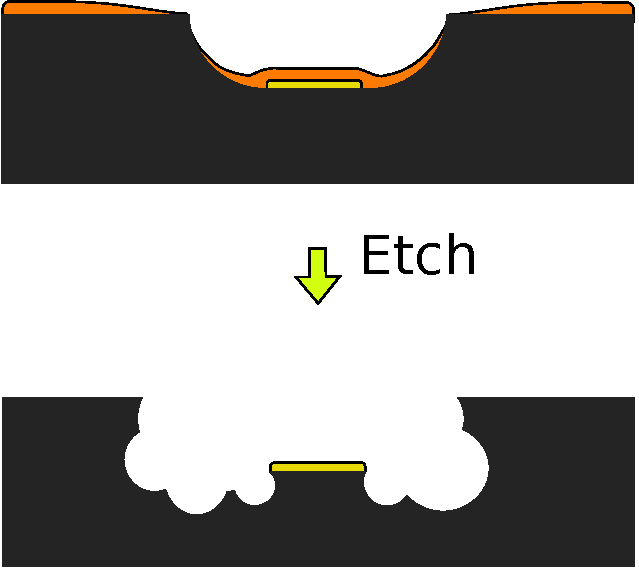
\includegraphics[width=\linewidth]{images/pmmacoverage.pdf} 
        \caption{PMMA step coverage} \label{fig:lil}
    \end{subfigure}
    \hfill
    \begin{subfigure}[ht]{0.48\textwidth}
        \centering
        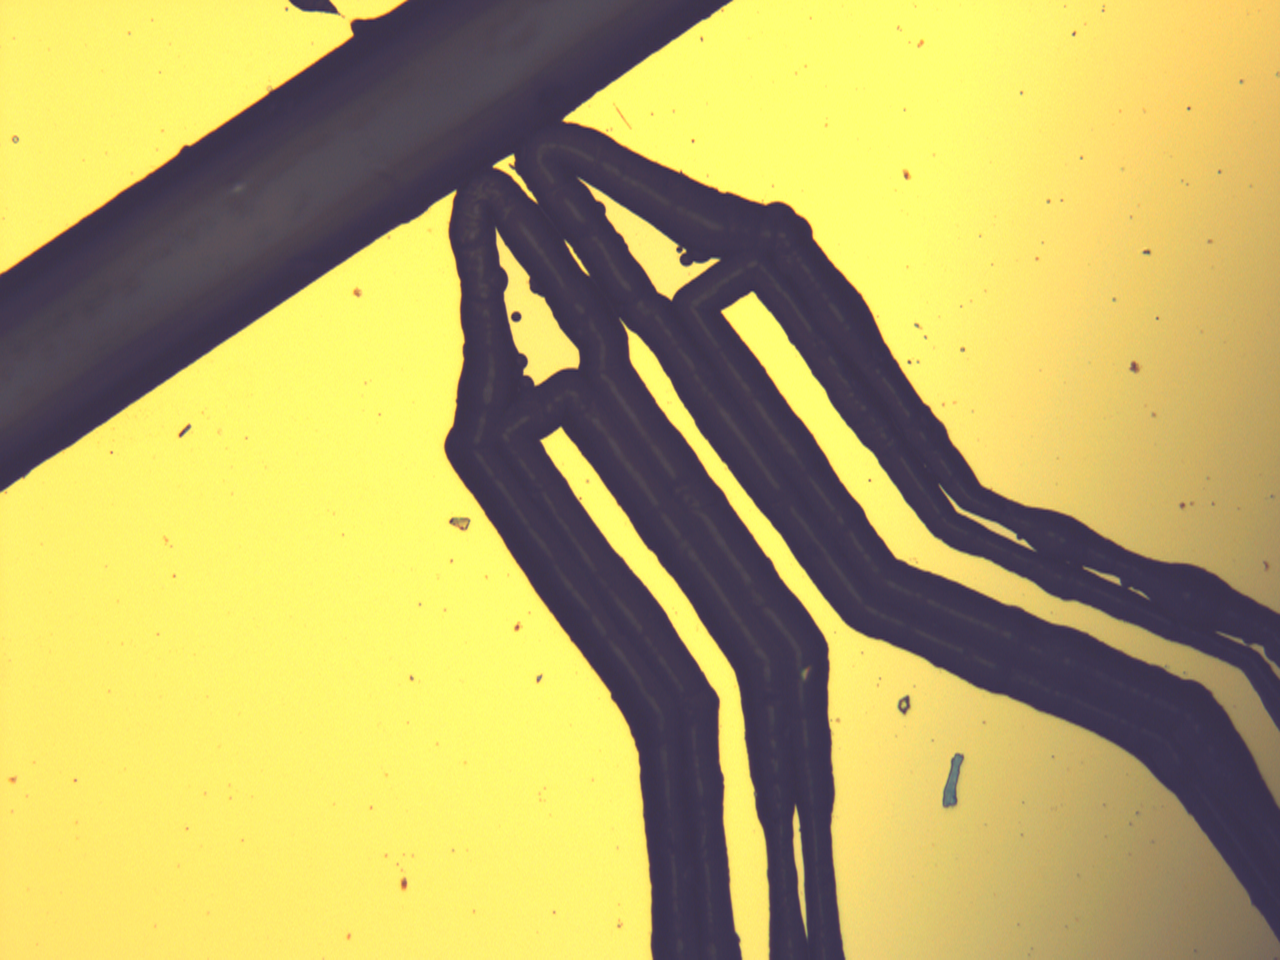
\includegraphics[width=\linewidth]{optical/electrodesideetch.png} 
        \caption{Unwanted etching of sharp features} \label{fig:lell}
    \end{subfigure}
    \caption{Using a PMMA layer thinner than electrode depth or not evaporating at an angle will cause sharp edges to be etched.} \label{fig:coverage}
\end{figure}  


Arguably, the problem of covering properly the $\SI{30}{\micro \metre}$ deep channels could have been solved using a photoresist and photolithography or by spray coating PMMA to have ideal step coverage. These methods not being readily available at the facility, the second option was chosen, which was to manufacture the electrodes first. \textcolor{red}{should this even be mentioned?}
Fabricating the electrodes firs meant that they need to be capable of withstanding the etching of the deep main-channels and the removal of the Cr-Au mask. Shallow (1-2$\; \micro \metre$) deep channels were etched for the electrodes using a $\SI{100}{\nano \metre}$ chromium mask. The electrode material could be then deposited without removing the etch mask. This meant that the electrode material ha a “double lift-off” by the removal of the resist and the Cr-mask. It made sure that no unwanted electrode material was left on the surface. The shallow depth also allowed the use of PMMA. Spin coating PMMA A11 at 3000 rpm results in a thickness of $\SI{2.25}{\micro \metre}$, which grants complete coverage of the electrodes. Evaporation of the deep-etch Cr/Au mask at $45^{\circ}$ with wafer rotation ensured mask coverage as well.


For the removal of the Cr-mask, a Nichrome etchant was used. Its selectivity was ideal; not harming the electrodes in any way \cite{williams2003etch}. This property was also exploited for the removal of the deep-etch mask. On top of the electrodes a Cr-Au was evaporated. After etching, the mask could be removed by using solely the Nichrome etchant. Using a gold etchant could have harmed the electrodes (also consisting of gold). 

The “lift-off” of the gold mask happened a lot faster (5 min) than expected from the etch rate of nichrome etchant ($\SI{50}{\angstrom \per \sec}$ at $\SI{40}{\celsius}$). It was expected to last a long time, considering the large area of $20\times 20\; \milli \metre$. This is speculated due to an electrochemical effect between the Au/Cr interface and the etchant solution, which has been demonstrated by Nemirovsky et al. for undercutting of Au when iodine etchants are used. Although in this case beneficial, the fast under etching of the Cr layer caused destruction of the electrodes in a few experiments (Figure \ref{fig:underetch}). Another reason could be the stress within the deposited gold film. The tensile lifting the gold could lead to the detachment and peeling of either the Au/Cr or the Cr/glass interface allowing the Cr-etchant to etch the underlying chromium (Figure \ref{fig:underetch}).

\begin{figure}[h]
    \centering
    \begin{subfigure}{0.48\textwidth}
        \centering
        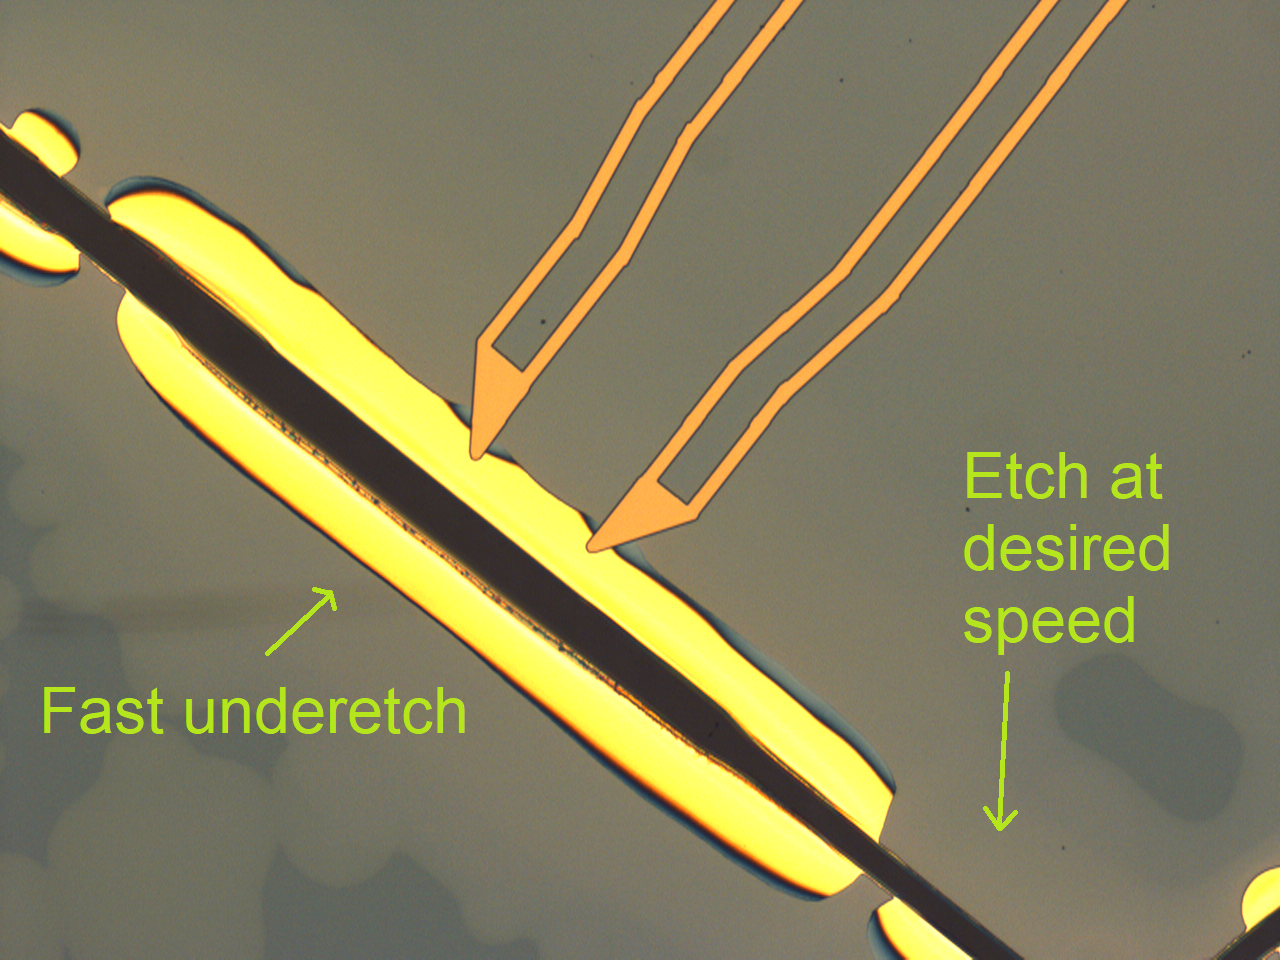
\includegraphics[width=\linewidth]{optical/underetch01.png} 
        \caption{} \label{fig:lileee}
    \end{subfigure}
    \hfill
    \begin{subfigure}{0.48\textwidth}
        \centering
        
\includegraphics[width=\linewidth]{optical/tensilestress.png} 
        \caption{} \label{fig:lellqqq}
    \end{subfigure}
    \caption{Over etching of Cr under Au mask. 1) The fast under etching of Cr ruined the electrodes. (Image taken from the bottom of the chip.) 2) Tensile stress visible when the gold mask is peeling upwards after channel etch.} \label{fig:underetch}
\end{figure}  


\textcolor{red}{desicion toward end}
(Should the electrode blistering be talked about?  Compressive stress? Bubbling of the gold but the cR being attached to the glass)

\newpage

\begin{flushleft}\textbf{Composition} \end{flushleft}
Besides good conductivity, the requirements for the electrode composition arise from the chip fabrication steps. The electrodes need to withstand:
\begin{enumerate}
    \renewcommand{\labelenumi}{\Roman{enumi}} 
    \setlength{\itemsep}{1pt}
    \setlength{\parskip}{1pt}
    \item The etchants used in lift-off
    \item Good adhesion to glass, for cleaning steps (sonication)
    \item Can endure Piranha treatment for chip activation (for TADB)
    \item Thermal endurance; not melting and retaining conductivity after being subjected for 590$\celsius$ in TADB
    \item Can be soldered to connecting wires
\end{enumerate}

An electrode composition meeting the requirements had already been demonstrated by Borovsky \cite{borovsky}; It was a sandwich of $\mathrm{SiO_{2}}$, Ti, Au, Ti and $\mathrm{SiO_{2}}$. Gold was chosen because its ideal conductivity and chemical resistance. As an adhesion layer between gold and glass, titanium was chosen. Although Ti is a slightly weaker adhesion layer than Cr \cite{chen2013study}, the annealing temperature in TADB causes chromium to diffuse into gold increasing its resistance significantly \cite{huang2003effect}. Titanium will also diffuse through Gold forming  $\mathrm{TiAu_2}$, TiAu and  $\mathrm{Ti_3 Au}$ compounds. The $\mathrm{Ti_3 Au}$ will  forms a thin (50-$\SI{100}{\angstrom}$) diffusion barrier preventing further diffusion \cite{tisone1972diffusion}. The initial $\mathrm{SiO_2}$ layer was designed to prevent diffusion between Ti and Glass which would lead to defective electrodes.  The first $\mathrm{SiO_2}$ layer was deemed unnecessary and working electrodes were manufactured without it. Adhesion problems between the deposited $\mathrm{SiO_2}$ and the electrodes drove towards this decision (Figure \ref{fig:eleproblem}). It can be speculated that the first $\mathrm{SiO_2}$ layer is indeed mandatory if the electrodes are placed between glass slides and subjected to pressure. The pressure may have lead to melting point depression and increased diffusion, which was not the case with our imbedded electrodes. After TADB a slight change in electrode colour was observed but the electrode resistance ($\SI{800}{\ohm}$ to $\SI{1}{\kilo \ohm}$) was not affected.
To further improve adhesion and to avoid Ti oxidation, all of the electrode material was evaporated consecutively. The final layer ($\mathrm{SiO_2}$), which served a purpose of protecting the electrodes against Piranha treatment (Figure \ref{fig:eleproblem}), made the electrode surface non-conductive. As a final processing step after cover-glass bonding, this layer was etched away using a RIE oxide etch. This etch did not visibly alter the glass cover transparency.


\begin{table}[h]
    \centering
    \caption{The final electrode composition.}
    \label{tab:electrde}
    \begin{tabular}{||c c c p{10cm}||} \toprule
       Order    & Material & Thickness & Purpose\\ \midrule
       (1)   &  Ti  &  $\SI{10}{\nano \metre}$  & An adhesion layer between Glass and Gold     \\ \hline
       (2)  &  Au  &  $\SI{50}{\nano \metre}$ & A long lasting and chemically resistive conductor \\\hline
       (3)  &  Ti  &  $\SI{10}{\nano \metre}$ & An adhesion layer between Gold and the protective layer of Silicon dioxide\\\hline
       (4)   &  $\mathrm{SiO_2}$  &  $\SI{100}{\nano \metre}$  & Acts as a protective layer against corrosive chemical treatments and separates electrodes from masking metal films    \\
         \bottomrule
    \end{tabular}
 \end{table}


 \begin{figure}
    \centering
    \begin{subfigure}[ht]{0.48\textwidth}
        \centering
        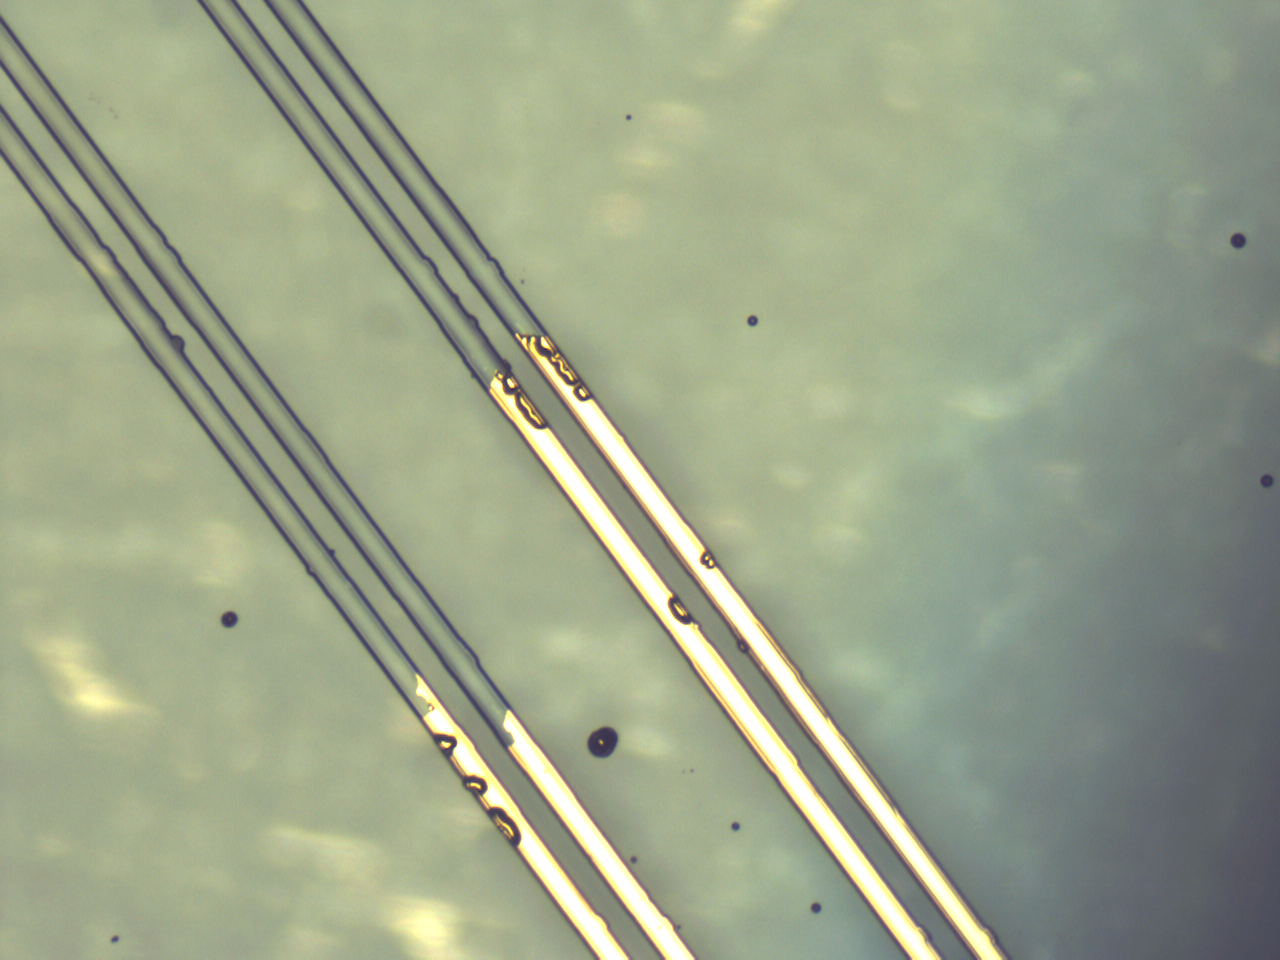
\includegraphics[width=\linewidth]{optical/eledetach.png} 
        \caption{} \label{fig:lileee}
    \end{subfigure}
    \hfill
    \begin{subfigure}[ht]{0.48\textwidth}
        \centering
        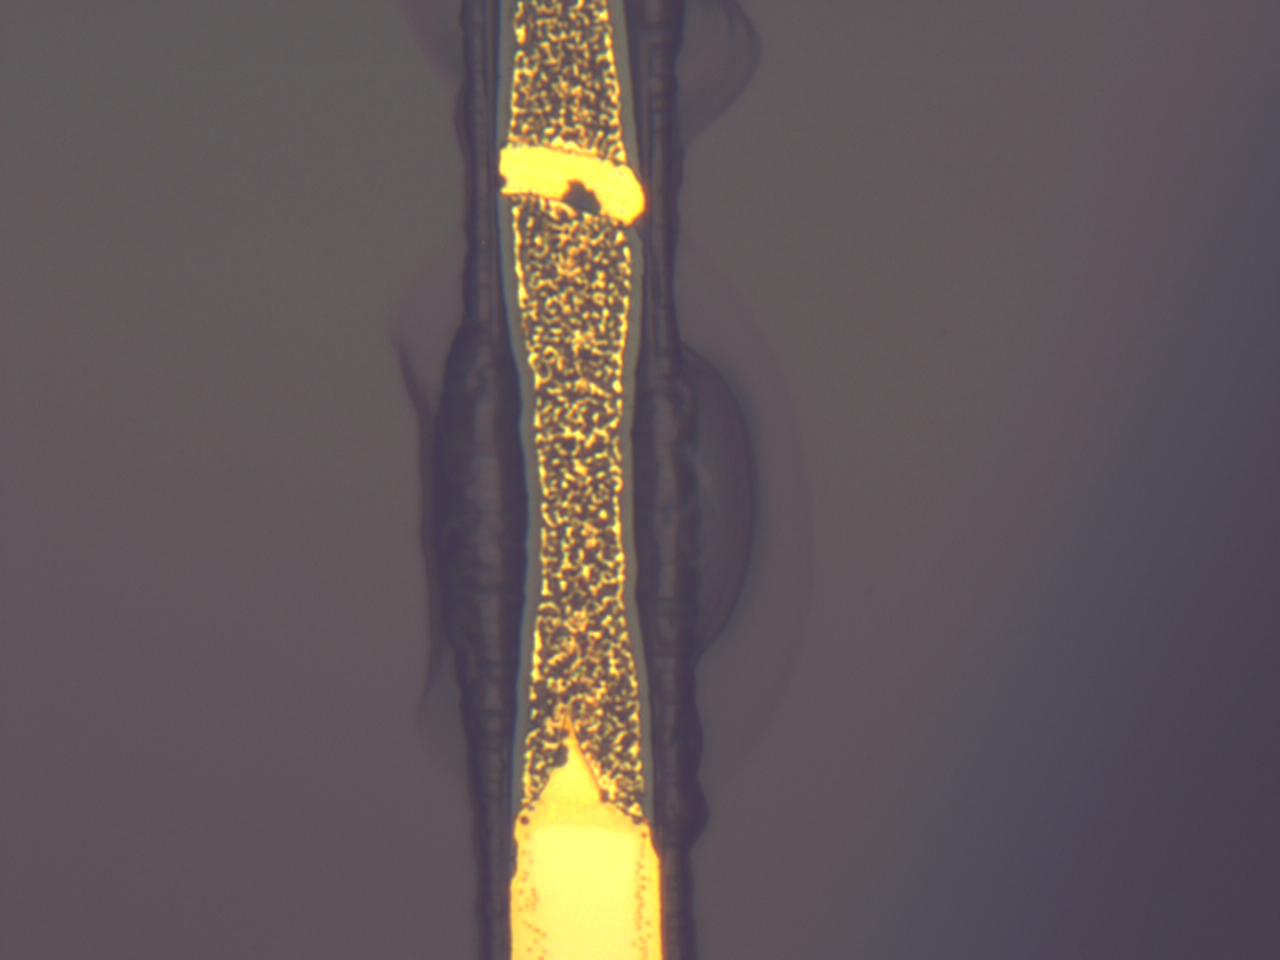
\includegraphics[width=\linewidth]{optical/piranha_ate.png} 
        \caption{} \label{fig:lellqqq}
    \end{subfigure}
    \caption{1) Electrodes detaching from glass due to bad adhesion. 2) HF etched the protective $\mathrm{SiO_2}$ layer through a pinhole, which lead to piranha corroding the gold.} \label{fig:eleproblem}
\end{figure}  



\textcolor{red}{(Should blisters in electrodes be talked about?)}



\subsection{Experiment setup}
\label{sec:xxx5}
\begin{itemize}
    \item Microfluidic setup (images, and illustrative image of pressure pumping method)
    \item How the laser + high voltage was set-up (circuit diagram)
    \item images of progression, challenges that were faced
\end{itemize}



\section{Measurements (and results?)}
\label{sec:results}
\begin{itemize}
    \item flow speed (TO BE MEASURED)
    \item DEP setup, voltage and frequency tests, maybe even electrode distance (TO BE MEASURED)
    \item Deflection of fluorescent beads, maybe even cells (TO BE MEASURED)
\end{itemize}

\begin{figure}
    \centering
    \begin{subfigure}[ht]{0.48\textwidth}
        \centering
        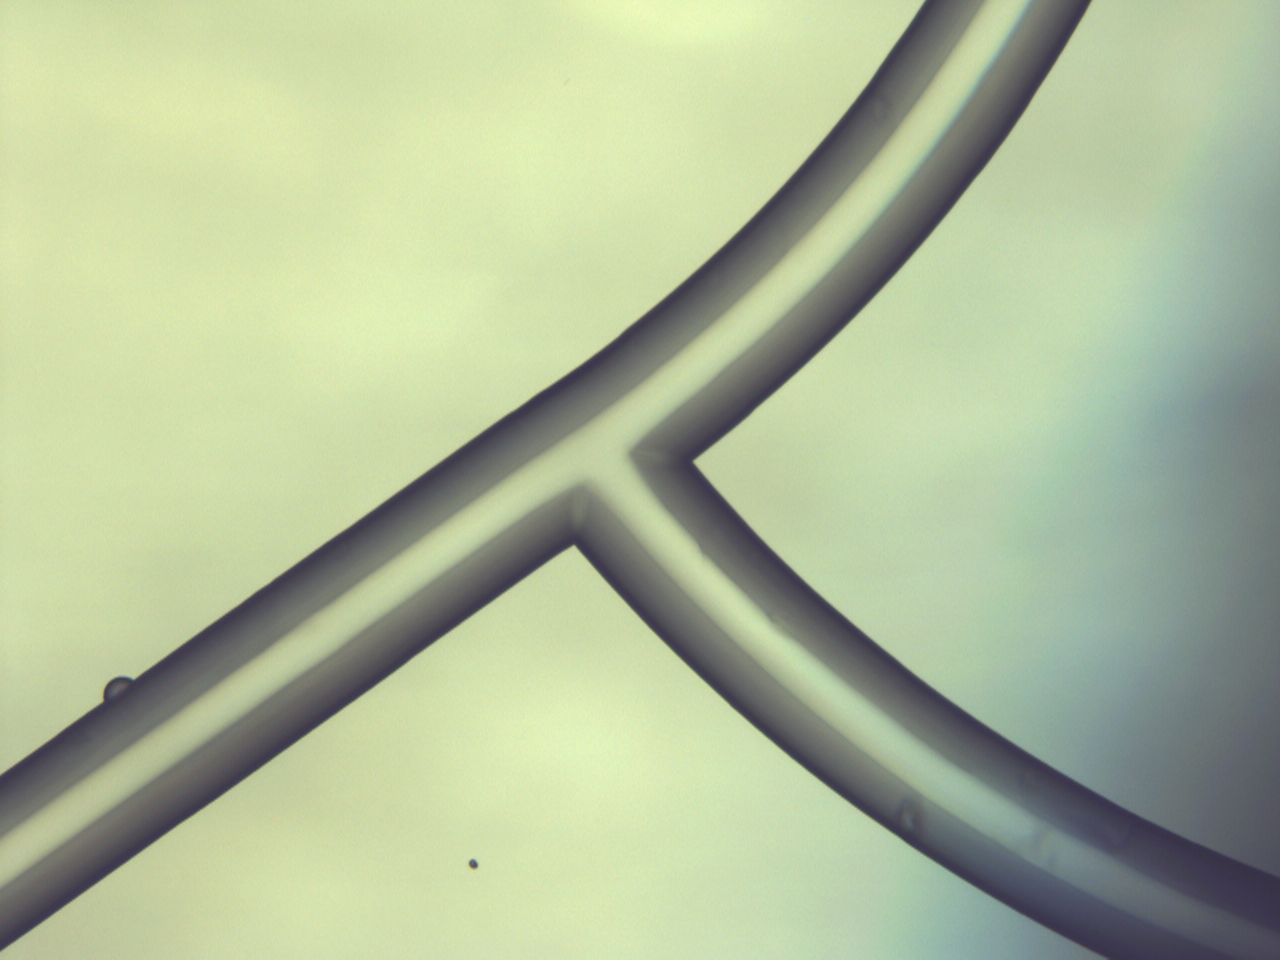
\includegraphics[width=\linewidth]{optical/good2.png} 
        \caption{} \label{fig:lileee}
    \end{subfigure}
    \hfill
    \begin{subfigure}[ht]{0.48\textwidth}
        \centering
        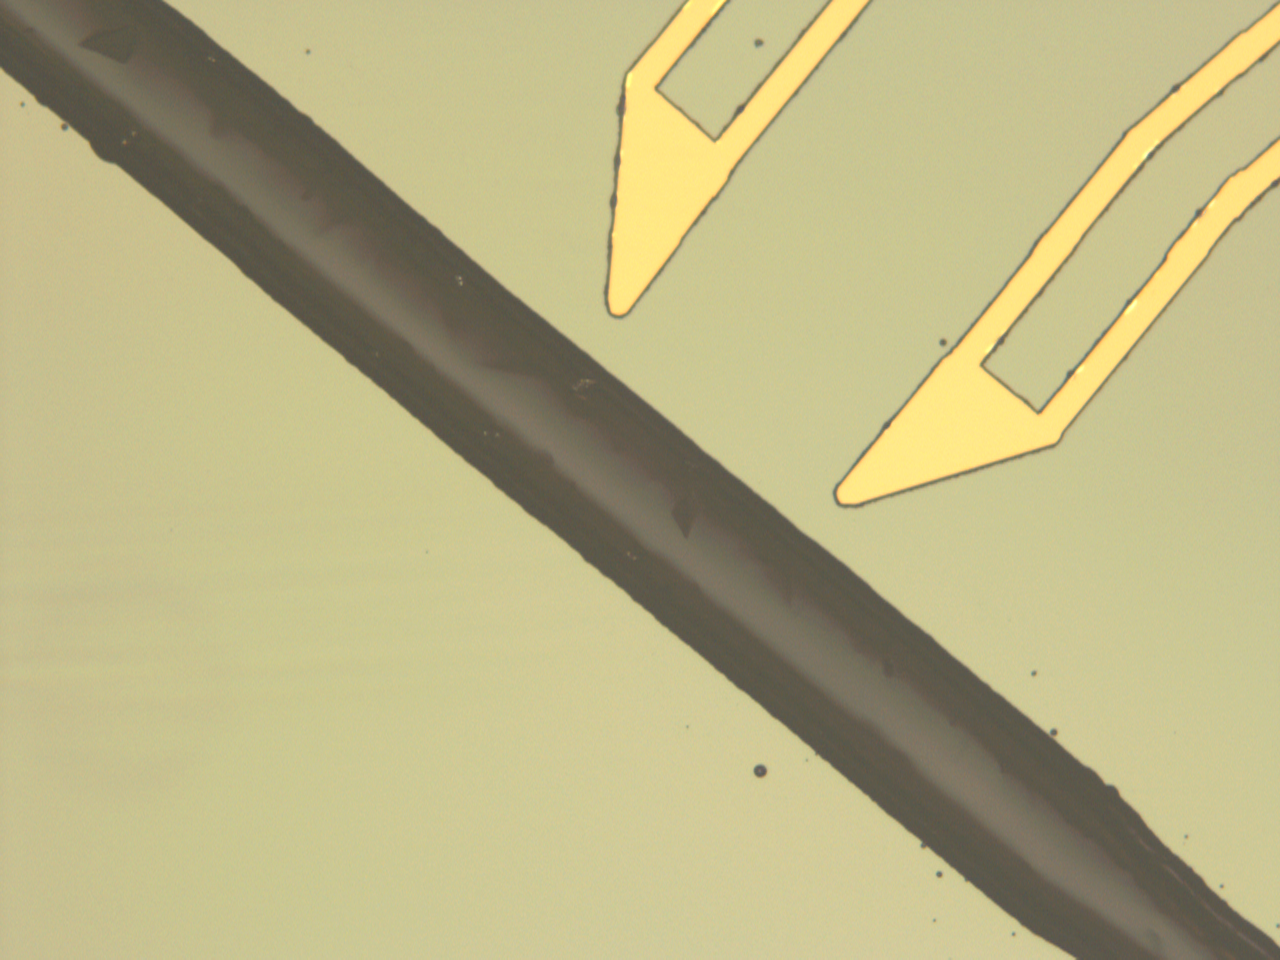
\includegraphics[width=\linewidth]{optical/good5.png} 
        \caption{} \label{fig:lellqqq}
    \end{subfigure}
    \caption{Add some of these final "good" result images.} \label{fig:ghj}
\end{figure}  
\section{Conclusions}
\label{sec:conclusions}


Conclusions

\nocite{*}

% --------------------------------------------------------------------------
% LÄHTEET
% --------------------------------------------------------------------------
%\printbibheading[heading=bibintoc]
\printbibliography
% --------------------------------------------------------------------------
% LIITTEET
% --------------------------------------------------------------------------
\appendix

\section{Appendix}
\label{sec:chemicals}

\begin{table}[h]
    \centering
    \caption{Chemicals information.}
    \label{tab:chemicals}
    \begin{tabular}{||l l l||} \toprule
       \textbf{Use case}    & \textbf{Name} & \textbf{Manufacturer} \\ \midrule
       Au etching   & Gold Etchant, Standard 651818-500ml  &  Sigma Aldrich \\ \hline
       Cr etching  &  Nichrome etchant 651834-500ml  &  Sigma Aldrich \\\hline
       Glass etching  &  Hydrofluoric acid $48\percent$  &  EMSURE \\\hline
       Glass etching   &  Hydrochloric acid $37\percent$  & AnalaR, NORMAPUR \\\hline
       Piranha solution & Sulfuric acid $95-97\percent$ & EMSURE \\\hline
       Piranha solution & Hydrogen peroxide $30\percent$ & AnalaR, NORMAPUR \\\hline
       EBL-resist & PMMA 950K A11 & Allresist \\\hline
       EBL-resist (conductive) & Electra 92 (AR-PC 5090) & Allresist \\\hline
         \bottomrule
    \end{tabular}
 \end{table}


\section{Appendix}
\label{sec:appendix2}
Steps marked between with the same colour must be done consecutively during the same day.
*Developer1 = MIBK:IPA*

1. (\textbf{Drilling}) Drill chip inlets and outlets using a Laser or mechanical drill bits.

2. (\textbf{Annealing}) Start with 3-4 chips for time efficiency. Sonicate and scrub with cotton tips in acetone and rinse with IPA. After drying with $\mathrm{N_2}$-gun, put the chips in the furnace within the sample holder. Set Dwelling time 6h on $560\celsius$ and make sure there is an $\mathrm{N_2}$ flow within the furnace. When heating and cooling the furnace is set to $\SI{4}{\celsius  \per \min}$.

\textcolor{orange}{3. (\textbf{Cleaning})} Take two flat beakers with Acetone and put one on a hotplate to boil. In the cool acetone, scrub chips with cotton tips holding them down with tweezers. Rinse with fresh acetone and put into the boiling one and Sonicate for 2 min. Repeat this step until no visible contamination/dust particles are present when dried with $\mathrm{N_2}$. Then Sonicate in IPA for 1 min and rinse with fresh IPA and put into $\mathrm{dH_2 O}$.

\textcolor{orange}{4. (\textbf{Activation})} Prepare a big and a small beaker filled with $\mathrm{dH_2 O}$ and a beaker for piranha. Set hotplate to $\SI{100}{\celsius}$. Use acid gloves and metal tweezers! Pour Sulphuric acid ($\mathrm{H_2 SO_4}$) FIRST! and then Hydrogen Peroxide ($\mathrm{H_2 O_2}$) in a ration of 3:1. (For a flat beaker $\SI{6}{\milli \litre}$ $\mathrm{H_2 SO_4}$ and $\SI{2}{\milli \litre}$ $\mathrm{H_2 O_2}$ is enough to cover the chips). Pipet $\mathrm{H_2 O_2}$ slowly to avoid a too strong reaction and fast release of gases. Wait until the exothermic reaction has cooled and put it on the hot plate. Dry chips with $\mathrm{N_2}$ and put in piranha for 30 min, lifting them with tweezers from time to time to remove bubbles. Dip chips into $\mathrm{dH_2 O}$ and rinse under flowing $\mathrm{dH_2 O}$ properly. Put into beaker with $\mathrm{dH_2 O}$. When all chips are rinsed, Put back to piranha for 5 min. When done, wash the chips under flowing $\mathrm{dH_2 O}$ thoroughly, making sure that no piranha is left in the drilled holes. Contain chips in $\mathrm{dH_2 O}$.

\textcolor{orange}{5. (\textbf{Evaporation, Mask})} Prepare evaporator fully; Clean crucibles and target materials ready, chamber de-vacuumed. In laminar flow room, dry chips with $\mathrm{N_2}$ and put on hot plate $130\celsius$ for 2 min to evaporate any moisture on chip surface. Put chips in evaporator (Care! High chance of contaminating chips!). Evaporate $\SI{100}{\nano \metre}$ of Cr with a slow rotation of the substrate.


\textcolor{purple}{6. (\textbf{Spin-coating})} Properly blow chips with $\mathrm{N_2}$ and put on hotplate 2 min $160 \celsius$ to remove moisture. Let chip cool on a clean aluminium block and blow with $\mathrm{N_2}$. Place chip in spin coater and turn on suction. Pipette PMMA 950K A4 evenly on the chip, making sure there are no bubbles present. Use pipette to remove possible bubbles. Spin at 3000 rpm for $\SI{60}{\second}$ with a ramp up speed of 500 rpm/s. Postbake on $160 \celsius$ for 2 min to remove PMMA solvent and cool chip on an aluminium block.

\textcolor{purple}{7. (\textbf{Exposure, Electrodes})} Scratch PMMA off a small area near where the evaporator holder was, to get the e-beam holder clamp in contact with the metal mask. Otherwise, serious charging and destruction of the resist might occur. You can scratch the mask also to generate “metal dust” that can be used for write field alignment. Set $\SI{120}{\micro \metre}$ aperture with $\SI{200}{\kilo \volt}$, because large areas are to be exposed. The beam current should measure about $\SI{10}{\nano \ampere}$. Use angle correction to align the pattern layout to the chip corners (avoiding any unnecessary exposure). Preform wright field alignment and expose Electrode layout, using a area dose of $\SI{215}{\micro \coulomb \per \centi\metre^2}$. Develop in Developer1 for 40s and then stir in IPA for 10s to stop and flush any developer on the chip. The chips were then Hardbaked at $180 \celsius$ for 1h.

8. (\textbf{Etching}) The mask ($\SI{100}{\nano \metre}$ Cr) is etched by submerging the chip in Cr-etchant at $40 \celsius$ gently shaking for 25s, then dipping and rinsing with $\mathrm{dH_2 O}$. Put on HF-protective gear and prepare chemicals and equipment for HF-etch. Pour $18\;$ml of HF and pipette (glass) 2 ml of HCL and mix them with HF-tweezers. Dip the chip in HF for 2s and stop in $\mathrm{dH_2 O}$. Rinse in $\mathrm{dH_2 O}$ and store chips in fresh $\mathrm{dH_2 O}$. 

\textcolor{orange}{9. (\textbf{Cleaning})}. An edge of a cleanroom sheet can be used to absorb water from the hydrophobic surface and then dry Gently with $\mathrm{N_2}$. Treat the chips with RIE $\mathrm{O_2}$ clean (60W for 45s) to remove any PMMA contaminants from electrode channels and to reactivate surface. Store chips in $\mathrm{dH_2 O}$.

\textcolor{orange}{10. (\textbf{Evaporation, electrodes})} Prepare evaporator fully; Clean crucibles and target materials ready, chamber de-vacuumed. In laminar flow room, dry chips with $\mathrm{N_2}$ and put on hot plate $130 \celsius$ for 2 min to evaporate any moisture on chip surface. Put chips in evaporator (Care! High chance of contaminating chips!). Evaporate $\SI{10}{\nano \metre}$ Ti + $\SI{50}{\nano \metre}$ Au + $\SI{10}{\nano \metre}$ Ti + $\SI{100}{\nano \metre}$ $\mathrm{SiO_2}$ with no rotation and 0 angle. 


11. (\textbf{Lift-off}) Remove PMMA in acetone, Don’t sonicate electrodes! Use Cr-etchant to remove the fully remove the mask. Make sure no residues are left in chip where they would matter. If must, sonication and mechanical scrubbing might be applied at the risk of destroying the electrodes. 

\textcolor{purple}{12. (\textbf{Activation, RIE})} Rinse chips with $\mathrm{dH_2 O}$ and dry with $\mathrm{N_2}$ blowing. Treat chips with RIE $\mathrm{O_2}$ clean (200 W, 2 min, 40 mTorr). Contain chips in $\mathrm{dH_2 O}$.

\textcolor{purple}{13. (\textbf{Evaporation, Mask})} Prepare evaporator fully; Clean crucibles and target materials ready, chamber de-vacuumed. In laminar flow room, dry chips with $\mathrm{N_2}$ and put on hot plate $130 \celsius$ for 2 min to evaporate any moisture on chip surface. Put chips in evaporator (Care! High chance of contaminating chips!). Using slow rotation at $45^{\circ}$ angle, evaporate $\SI{50}{\nano \metre}$ Cr wait 5 min, $\SI{200}{\nano \metre}$ Au, wait 10 min, $\SI{100}{\nano \metre}$ Au. Don’t evaporate Au over $\SI{1.2}{\angstrom \per \sec}$ or it will deposit large chunks wasting gold and reducing mask quality.

\textcolor{orange}{14. (\textbf{Spin-coating})} Properly blow chips with $\mathrm{N_2}$ and put on hotplate 2 min $160 \celsius$ to remove moisture. Let chip cool on a clean aluminium block and blow with $\mathrm{N_2}$. Place chip in spin coater and turn on suction. Pipette PMMA 950K A11 evenly on the chip, making sure there are no bubbles present. Use pipette to remove possible bubbles. Spin at 3000 rpm for 60s with a ramp up speed of 500 rpm/s. Postbake on $160\celsius$ for 3 min to remove PMMA solvent and cool chip on an aluminium block.

\textcolor{orange}{15. (\textbf{Exposure, Channels})} Same procedure as in step 5. Preform wright field alignment and expose Channel layout, using a area dose of $\SI{450}{\micro \coulomb \per \centi\metre^2}$. Develop in Developer1 for 55s and then stir in IPA for 10s to stop and flush any developer on the chip. 

16. (\textbf{Etching}) Protect the electrodes by covering them with tape. The mask ($\SI{50}{\nano \metre}$ Cr + $\SI{200}{\nano \metre}$ Au) is etched by submerging the chip in Au-etchant for 25s and gently shaking, stop in $\mathrm{dH_2 O}$. Next, dip in Cr-etchant  for 10s 40$\celsius$ gently shaking then dipping and rinsing with $\mathrm{dH_2 O}$. Check under microscope, make sure Cr  etchant didn’t under etch the Au mask by inspecting the chip upside-down under a microscope. Put on HF-protective gear and prepare chemicals and equipment for HF-etch. Pour 18 ml of HF and pipette (glass) 2 ml of HCL and mix them with HF-tweezers. Dip the chip in HF for 55s gently stirring and stop in $\mathrm{dH_2 O}$. Rinse in $\mathrm{dH_2 O}$ and remove PMMA in Acetone. Lift-off Au-mask using hot Cr-etchant. Mechanical help with tweezers should be applied to remove Au-mask. Rinse in $\mathrm{dH_2 O}$.

17. (\textbf{TDAB}) This step is extremely susceptible to contamination, try to minimize contamination at all means (wear proper face mask etc.). Remember which side of the glass is to be bonded to avoid contaminating it. The chip and the $18\times18 \; \milli \metre^2$ coverslip is prepared for bonding.

\textbf{For cover:}
Take 2x cover glass. Scrub and sonicate (5 min) in hot acetone. Redo with fresh acetone and then rinse and sonicate (1 min) in IPA. Blow dry with $\mathrm{N_2}$. Preform activation as in step 4. Keep to be bonded side upwards. Sonicate in $\mathrm{dH_2 O}$ for 5 min and put into fresh $\mathrm{dH_2 O}$.

\textbf{For chip with channels:}
(If “blisters” are present in electrodes, sonication will destroy them!) Rinse and Sonicate upside down (electrodes facing beaker bottom) for 30s in acetone. Rinse and sonicate 10s in IPA. (Sonication time is a trade-off between successful TDAB and destroyed electrodes). Keep in $\mathrm{dH_2 O}$ until activation. Dry with $\mathrm{N_2}$ and Treat in fresh Room temperature piranha for (7 + 3) min rinsing with $\mathrm{dH_2 O}$ in between. Keep to be bonded side upwards. Before rinsing put in $\mathrm{dH_2 O}$ beaker first! Any piranha solution between tweezers and chip can cause it to slip and drop during rinsing! Contain chips in $\mathrm{dH_2 O}$.\newline

Rinse the chips in $\mathrm{dH_2 O}$ and dry with $\mathrm{N_2}$ under laminar flow hood and put them on hotplate 130$\celsius$ for 2 min in laminar flow room. Cool chips on a clean Al-block. With the help of a tweezer, grab the back of the cover glass and place it on top of the channels-chip. To remove all newton-rings the glasses can be pushed together with your thumb. A force at full strength can be applied, IF the chip is on a completely flat solid surface. If newton rings still remain, or the glasses don’t stick together, the whole process step 17 needs to be redone. A properly bonded glass looks as of being one unit. Place the chip cover upwards into the stainless steel holder and put the weight on top. Place the holder in the furnace and set dwell time 585$\celsius$ for 2h under nitrogen flow.

18.(\textbf{Finish}) Lastly, the protective layer ($\mathrm{SiO_2}$) on top of the electrodes will be removed. Treat the chip with RIE Oxide Etch (O2 -flash at 30$\celsius$ for 4 min (Etches $\SI{42}{\nano \metre \per \min}$). This will remove the top layer of protective $\mathrm{SiO_2}$ on the electrode pads and make them conductive.





\end{document}

